%# -*- coding: utf-8 -*-
%!TEX encoding = UTF-8 Unicode
%!TEX TS-program = xelatex
% vim:ts=4:sw=4
%
% 以上设定默认使用 XeLaTex 编译,并指定 Unicode 编码,供 TeXShop 自动识别

% Author: Yunhui Fu <yhfudev@gmail.com>
% License: Creative Commons (CC BY 4.0)

\section{\cnt{Sparse Autoencoder}{稀疏自编码器}{}}

\subsection{\cnt{Neural Networks}{神经网络}{}} \label{chp:neuralnet}


\cnt{Consider a supervised learning problem where we have access to labeled training examples $(x^{(i)},y^{(i)})$. Neural networks give a way of defining a complex, non-linear form of hypotheses $h_{W,b}(x)$, with parameters $W,b$ that we can fit to our data.}
    {以监督学习为例,假设我们有训练样本集 $(x^{(i)},y^{(i)})$,那么神经网络算法能够提供一种复杂且非线性的假设模型 $h_{W,b}(x)$,它具有参数 $W, b$,可以以此参数来拟合我们的数据。}
    {}

\cnt{To describe neural networks, we will begin by describing the simplest possible neural network, one which comprises a single ``neuron." We will use the following diagram to denote a single neuron:}
    {为了描述神经网络,我们先从最简单的神经网络讲起,这个神经网络仅由一个“神经元”构成,以下即是这个“神经元”的图示:}
    {}


\begin{figure}[ht] \centering
  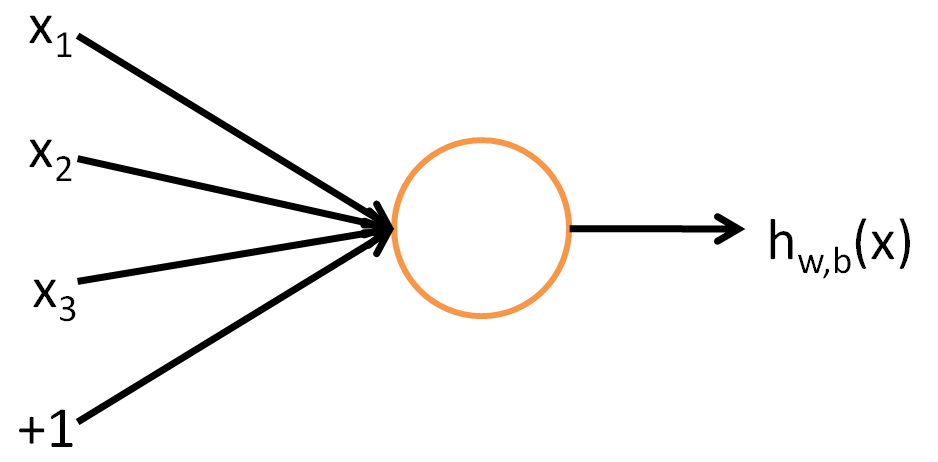
\includegraphics[width=0.5\textwidth]{figures/SingleNeuron.png}
  %\caption{}\label{fig:step1}
\end{figure}


\cnt{This ``neuron\index{neuron}" is a computational unit that takes as input $x_1,x_2,x_3$ (and a +1 intercept term), and outputs $h_{W,b}(x) = f(W^Tx) = f(\sum_{i=1}^3 W_{i}x_i +b)$, where $f : \Re \mapsto \Re$ is called the \emph{activation function}\index{activation function}. In these notes, we will choose $f(\cdot)$ to be the \index{sigmoid} function:}
    {这个“神经元\index{神经元}”是一个以 $x_1, x_2, x_3$ 及截距 $+1$ 为输入值的运算单元,其输出为 $h_{W,b}(x) = f(W^Tx) = f(\sum_{i=1}^3 W_{i}x_i +b)$,其中函数 $f : \Re \mapsto \Re$ 被称为“激活函数\index{激活函数}”。在本教程中,我们选用 sigmoid\index{sigmoid} 函数作为\emph{激活函数} $f(\cdot)$}
    {}

$$
f(z) = \frac{1}{1+\exp(-z)}.
$$

\cnt{Thus, our single neuron corresponds exactly to the input-output mapping defined by logistic regression.}
    {可以看出,这个单一“神经元”的输入-输出映射关系其实就是一个逻辑回归(logistic regression)。}
    {}
\cnt{Although these notes will use the sigmoid function, it is worth noting that another common choice for $f$ is the hyperbolic tangent\index{hyperbolic tangent}, or $\tanh$\index{tanh@$\tanh$}, function:}
    {虽然本系列教程采用sigmoid函数,但你也可以选择 双曲正切函数\index{双曲正切函数}($\tanh$\index{tanh@$\tanh$}):}
    {}

$$
f(z) = \tanh(z) = \frac{e^z - e^{-z}}{e^z + e^{-z}},
$$

%\cnt{Here are plots of the sigmoid(Figure \ref{fig:actfuncsig}) and $\tanh$ (Figure\ref{fig:actfunctanh}) functions:}
%    {以下图 \ref{fig:actfuncsig} 和 图 \ref{fig:actfunctanh} 分别是sigmoid及tanh的函数图像}
%    {}
\cnt{Here are plots of the sigmoid and $\tanh$ functions (Figure \ref{fig:actfuncs}):}
    {以下图 \ref{fig:actfuncs} 分别是 sigmoid 及 tanh 的函数图像}
    {}
\begin{figure}[ht] \centering
  % GNUPLOT: LaTeX picture
\setlength{\unitlength}{0.240900pt}
\ifx\plotpoint\undefined\newsavebox{\plotpoint}\fi
\sbox{\plotpoint}{\rule[-0.200pt]{0.400pt}{0.400pt}}%
\begin{picture}(1500,900)(0,0)
\sbox{\plotpoint}{\rule[-0.200pt]{0.400pt}{0.400pt}}%
\sbox{\plotpoint}{\rule[-0.500pt]{1.000pt}{1.000pt}}%
\multiput(191,164)(20.756,0.000){44}{\usebox{\plotpoint}}
\put(1099,164){\usebox{\plotpoint}}
\put(1419.00,164.00){\usebox{\plotpoint}}
\put(1439,164){\usebox{\plotpoint}}
\sbox{\plotpoint}{\rule[-0.200pt]{0.400pt}{0.400pt}}%
\put(191.0,164.0){\rule[-0.200pt]{4.818pt}{0.400pt}}
\put(171,164){\makebox(0,0)[r]{-1}}
\put(1419.0,164.0){\rule[-0.200pt]{4.818pt}{0.400pt}}
\sbox{\plotpoint}{\rule[-0.500pt]{1.000pt}{1.000pt}}%
\multiput(191,330)(20.756,0.000){44}{\usebox{\plotpoint}}
\put(1099,330){\usebox{\plotpoint}}
\put(1419.00,330.00){\usebox{\plotpoint}}
\put(1439,330){\usebox{\plotpoint}}
\sbox{\plotpoint}{\rule[-0.200pt]{0.400pt}{0.400pt}}%
\put(191.0,330.0){\rule[-0.200pt]{4.818pt}{0.400pt}}
\put(171,330){\makebox(0,0)[r]{-0.5}}
\put(1419.0,330.0){\rule[-0.200pt]{4.818pt}{0.400pt}}
\sbox{\plotpoint}{\rule[-0.500pt]{1.000pt}{1.000pt}}%
\multiput(191,495)(20.756,0.000){61}{\usebox{\plotpoint}}
\put(1439,495){\usebox{\plotpoint}}
\sbox{\plotpoint}{\rule[-0.200pt]{0.400pt}{0.400pt}}%
\put(191.0,495.0){\rule[-0.200pt]{4.818pt}{0.400pt}}
\put(171,495){\makebox(0,0)[r]{ 0}}
\put(1419.0,495.0){\rule[-0.200pt]{4.818pt}{0.400pt}}
\sbox{\plotpoint}{\rule[-0.500pt]{1.000pt}{1.000pt}}%
\multiput(191,660)(20.756,0.000){61}{\usebox{\plotpoint}}
\put(1439,660){\usebox{\plotpoint}}
\sbox{\plotpoint}{\rule[-0.200pt]{0.400pt}{0.400pt}}%
\put(191.0,660.0){\rule[-0.200pt]{4.818pt}{0.400pt}}
\put(171,660){\makebox(0,0)[r]{ 0.5}}
\put(1419.0,660.0){\rule[-0.200pt]{4.818pt}{0.400pt}}
\sbox{\plotpoint}{\rule[-0.500pt]{1.000pt}{1.000pt}}%
\multiput(191,826)(20.756,0.000){61}{\usebox{\plotpoint}}
\put(1439,826){\usebox{\plotpoint}}
\sbox{\plotpoint}{\rule[-0.200pt]{0.400pt}{0.400pt}}%
\put(191.0,826.0){\rule[-0.200pt]{4.818pt}{0.400pt}}
\put(171,826){\makebox(0,0)[r]{ 1}}
\put(1419.0,826.0){\rule[-0.200pt]{4.818pt}{0.400pt}}
\sbox{\plotpoint}{\rule[-0.500pt]{1.000pt}{1.000pt}}%
\multiput(326,131)(0.000,20.756){36}{\usebox{\plotpoint}}
\put(326,859){\usebox{\plotpoint}}
\sbox{\plotpoint}{\rule[-0.200pt]{0.400pt}{0.400pt}}%
\put(326.0,131.0){\rule[-0.200pt]{0.400pt}{4.818pt}}
\put(326,90){\makebox(0,0){-4}}
\put(326.0,839.0){\rule[-0.200pt]{0.400pt}{4.818pt}}
\sbox{\plotpoint}{\rule[-0.500pt]{1.000pt}{1.000pt}}%
\multiput(570,131)(0.000,20.756){36}{\usebox{\plotpoint}}
\put(570,859){\usebox{\plotpoint}}
\sbox{\plotpoint}{\rule[-0.200pt]{0.400pt}{0.400pt}}%
\put(570.0,131.0){\rule[-0.200pt]{0.400pt}{4.818pt}}
\put(570,90){\makebox(0,0){-2}}
\put(570.0,839.0){\rule[-0.200pt]{0.400pt}{4.818pt}}
\sbox{\plotpoint}{\rule[-0.500pt]{1.000pt}{1.000pt}}%
\multiput(815,131)(0.000,20.756){36}{\usebox{\plotpoint}}
\put(815,859){\usebox{\plotpoint}}
\sbox{\plotpoint}{\rule[-0.200pt]{0.400pt}{0.400pt}}%
\put(815.0,131.0){\rule[-0.200pt]{0.400pt}{4.818pt}}
\put(815,90){\makebox(0,0){ 0}}
\put(815.0,839.0){\rule[-0.200pt]{0.400pt}{4.818pt}}
\sbox{\plotpoint}{\rule[-0.500pt]{1.000pt}{1.000pt}}%
\multiput(1060,131)(0.000,20.756){36}{\usebox{\plotpoint}}
\put(1060,859){\usebox{\plotpoint}}
\sbox{\plotpoint}{\rule[-0.200pt]{0.400pt}{0.400pt}}%
\put(1060.0,131.0){\rule[-0.200pt]{0.400pt}{4.818pt}}
\put(1060,90){\makebox(0,0){ 2}}
\put(1060.0,839.0){\rule[-0.200pt]{0.400pt}{4.818pt}}
\sbox{\plotpoint}{\rule[-0.500pt]{1.000pt}{1.000pt}}%
\put(1304.00,131.00){\usebox{\plotpoint}}
\put(1304,151){\usebox{\plotpoint}}
\multiput(1304,351)(0.000,20.756){25}{\usebox{\plotpoint}}
\put(1304,859){\usebox{\plotpoint}}
\sbox{\plotpoint}{\rule[-0.200pt]{0.400pt}{0.400pt}}%
\put(1304.0,131.0){\rule[-0.200pt]{0.400pt}{4.818pt}}
\put(1304,90){\makebox(0,0){ 4}}
\put(1304.0,839.0){\rule[-0.200pt]{0.400pt}{4.818pt}}
\put(191.0,131.0){\rule[-0.200pt]{0.400pt}{175.375pt}}
\put(191.0,131.0){\rule[-0.200pt]{300.643pt}{0.400pt}}
\put(1439.0,131.0){\rule[-0.200pt]{0.400pt}{175.375pt}}
\put(191.0,859.0){\rule[-0.200pt]{300.643pt}{0.400pt}}
\put(30,495){\makebox(0,0){$f(z)$}}
\put(815,29){\makebox(0,0){$z$}}
\put(1099.0,151.0){\rule[-0.200pt]{0.400pt}{48.180pt}}
\put(1099.0,351.0){\rule[-0.200pt]{77.088pt}{0.400pt}}
\put(1419.0,151.0){\rule[-0.200pt]{0.400pt}{48.180pt}}
\put(1099.0,151.0){\rule[-0.200pt]{77.088pt}{0.400pt}}
\put(1279,301){\makebox(0,0)[r]{$\frac{1}{1+\exp(-z)}$}}
\put(1299.0,301.0){\rule[-0.200pt]{24.090pt}{0.400pt}}
\put(191,497){\usebox{\plotpoint}}
\put(216,496.67){\rule{3.132pt}{0.400pt}}
\multiput(216.00,496.17)(6.500,1.000){2}{\rule{1.566pt}{0.400pt}}
\put(191.0,497.0){\rule[-0.200pt]{6.022pt}{0.400pt}}
\put(254,497.67){\rule{3.132pt}{0.400pt}}
\multiput(254.00,497.17)(6.500,1.000){2}{\rule{1.566pt}{0.400pt}}
\put(229.0,498.0){\rule[-0.200pt]{6.022pt}{0.400pt}}
\put(279,498.67){\rule{3.132pt}{0.400pt}}
\multiput(279.00,498.17)(6.500,1.000){2}{\rule{1.566pt}{0.400pt}}
\put(267.0,499.0){\rule[-0.200pt]{2.891pt}{0.400pt}}
\put(304,499.67){\rule{3.132pt}{0.400pt}}
\multiput(304.00,499.17)(6.500,1.000){2}{\rule{1.566pt}{0.400pt}}
\put(292.0,500.0){\rule[-0.200pt]{2.891pt}{0.400pt}}
\put(330,500.67){\rule{2.891pt}{0.400pt}}
\multiput(330.00,500.17)(6.000,1.000){2}{\rule{1.445pt}{0.400pt}}
\put(342,501.67){\rule{3.132pt}{0.400pt}}
\multiput(342.00,501.17)(6.500,1.000){2}{\rule{1.566pt}{0.400pt}}
\put(317.0,501.0){\rule[-0.200pt]{3.132pt}{0.400pt}}
\put(367,502.67){\rule{3.132pt}{0.400pt}}
\multiput(367.00,502.17)(6.500,1.000){2}{\rule{1.566pt}{0.400pt}}
\put(380,503.67){\rule{3.132pt}{0.400pt}}
\multiput(380.00,503.17)(6.500,1.000){2}{\rule{1.566pt}{0.400pt}}
\put(393,504.67){\rule{2.891pt}{0.400pt}}
\multiput(393.00,504.17)(6.000,1.000){2}{\rule{1.445pt}{0.400pt}}
\put(405,505.67){\rule{3.132pt}{0.400pt}}
\multiput(405.00,505.17)(6.500,1.000){2}{\rule{1.566pt}{0.400pt}}
\put(418,507.17){\rule{2.700pt}{0.400pt}}
\multiput(418.00,506.17)(7.396,2.000){2}{\rule{1.350pt}{0.400pt}}
\put(431,508.67){\rule{2.891pt}{0.400pt}}
\multiput(431.00,508.17)(6.000,1.000){2}{\rule{1.445pt}{0.400pt}}
\put(443,510.17){\rule{2.700pt}{0.400pt}}
\multiput(443.00,509.17)(7.396,2.000){2}{\rule{1.350pt}{0.400pt}}
\put(456,511.67){\rule{2.891pt}{0.400pt}}
\multiput(456.00,511.17)(6.000,1.000){2}{\rule{1.445pt}{0.400pt}}
\put(468,513.17){\rule{2.700pt}{0.400pt}}
\multiput(468.00,512.17)(7.396,2.000){2}{\rule{1.350pt}{0.400pt}}
\put(481,515.17){\rule{2.700pt}{0.400pt}}
\multiput(481.00,514.17)(7.396,2.000){2}{\rule{1.350pt}{0.400pt}}
\multiput(494.00,517.61)(2.472,0.447){3}{\rule{1.700pt}{0.108pt}}
\multiput(494.00,516.17)(8.472,3.000){2}{\rule{0.850pt}{0.400pt}}
\put(506,520.17){\rule{2.700pt}{0.400pt}}
\multiput(506.00,519.17)(7.396,2.000){2}{\rule{1.350pt}{0.400pt}}
\multiput(519.00,522.61)(2.472,0.447){3}{\rule{1.700pt}{0.108pt}}
\multiput(519.00,521.17)(8.472,3.000){2}{\rule{0.850pt}{0.400pt}}
\multiput(531.00,525.61)(2.695,0.447){3}{\rule{1.833pt}{0.108pt}}
\multiput(531.00,524.17)(9.195,3.000){2}{\rule{0.917pt}{0.400pt}}
\multiput(544.00,528.61)(2.695,0.447){3}{\rule{1.833pt}{0.108pt}}
\multiput(544.00,527.17)(9.195,3.000){2}{\rule{0.917pt}{0.400pt}}
\multiput(557.00,531.61)(2.472,0.447){3}{\rule{1.700pt}{0.108pt}}
\multiput(557.00,530.17)(8.472,3.000){2}{\rule{0.850pt}{0.400pt}}
\multiput(569.00,534.60)(1.797,0.468){5}{\rule{1.400pt}{0.113pt}}
\multiput(569.00,533.17)(10.094,4.000){2}{\rule{0.700pt}{0.400pt}}
\multiput(582.00,538.60)(1.651,0.468){5}{\rule{1.300pt}{0.113pt}}
\multiput(582.00,537.17)(9.302,4.000){2}{\rule{0.650pt}{0.400pt}}
\multiput(594.00,542.60)(1.797,0.468){5}{\rule{1.400pt}{0.113pt}}
\multiput(594.00,541.17)(10.094,4.000){2}{\rule{0.700pt}{0.400pt}}
\multiput(607.00,546.59)(1.378,0.477){7}{\rule{1.140pt}{0.115pt}}
\multiput(607.00,545.17)(10.634,5.000){2}{\rule{0.570pt}{0.400pt}}
\multiput(620.00,551.59)(1.267,0.477){7}{\rule{1.060pt}{0.115pt}}
\multiput(620.00,550.17)(9.800,5.000){2}{\rule{0.530pt}{0.400pt}}
\multiput(632.00,556.59)(1.378,0.477){7}{\rule{1.140pt}{0.115pt}}
\multiput(632.00,555.17)(10.634,5.000){2}{\rule{0.570pt}{0.400pt}}
\multiput(645.00,561.59)(1.033,0.482){9}{\rule{0.900pt}{0.116pt}}
\multiput(645.00,560.17)(10.132,6.000){2}{\rule{0.450pt}{0.400pt}}
\multiput(657.00,567.59)(1.378,0.477){7}{\rule{1.140pt}{0.115pt}}
\multiput(657.00,566.17)(10.634,5.000){2}{\rule{0.570pt}{0.400pt}}
\multiput(670.00,572.59)(0.950,0.485){11}{\rule{0.843pt}{0.117pt}}
\multiput(670.00,571.17)(11.251,7.000){2}{\rule{0.421pt}{0.400pt}}
\multiput(683.00,579.59)(1.033,0.482){9}{\rule{0.900pt}{0.116pt}}
\multiput(683.00,578.17)(10.132,6.000){2}{\rule{0.450pt}{0.400pt}}
\multiput(695.00,585.59)(0.950,0.485){11}{\rule{0.843pt}{0.117pt}}
\multiput(695.00,584.17)(11.251,7.000){2}{\rule{0.421pt}{0.400pt}}
\multiput(708.00,592.59)(0.758,0.488){13}{\rule{0.700pt}{0.117pt}}
\multiput(708.00,591.17)(10.547,8.000){2}{\rule{0.350pt}{0.400pt}}
\multiput(720.00,600.59)(0.950,0.485){11}{\rule{0.843pt}{0.117pt}}
\multiput(720.00,599.17)(11.251,7.000){2}{\rule{0.421pt}{0.400pt}}
\multiput(733.00,607.59)(0.824,0.488){13}{\rule{0.750pt}{0.117pt}}
\multiput(733.00,606.17)(11.443,8.000){2}{\rule{0.375pt}{0.400pt}}
\multiput(746.00,615.59)(0.758,0.488){13}{\rule{0.700pt}{0.117pt}}
\multiput(746.00,614.17)(10.547,8.000){2}{\rule{0.350pt}{0.400pt}}
\multiput(758.00,623.59)(0.824,0.488){13}{\rule{0.750pt}{0.117pt}}
\multiput(758.00,622.17)(11.443,8.000){2}{\rule{0.375pt}{0.400pt}}
\multiput(771.00,631.59)(0.758,0.488){13}{\rule{0.700pt}{0.117pt}}
\multiput(771.00,630.17)(10.547,8.000){2}{\rule{0.350pt}{0.400pt}}
\multiput(783.00,639.59)(0.728,0.489){15}{\rule{0.678pt}{0.118pt}}
\multiput(783.00,638.17)(11.593,9.000){2}{\rule{0.339pt}{0.400pt}}
\multiput(796.00,648.59)(0.824,0.488){13}{\rule{0.750pt}{0.117pt}}
\multiput(796.00,647.17)(11.443,8.000){2}{\rule{0.375pt}{0.400pt}}
\multiput(809.00,656.59)(0.669,0.489){15}{\rule{0.633pt}{0.118pt}}
\multiput(809.00,655.17)(10.685,9.000){2}{\rule{0.317pt}{0.400pt}}
\multiput(821.00,665.59)(0.824,0.488){13}{\rule{0.750pt}{0.117pt}}
\multiput(821.00,664.17)(11.443,8.000){2}{\rule{0.375pt}{0.400pt}}
\multiput(834.00,673.59)(0.728,0.489){15}{\rule{0.678pt}{0.118pt}}
\multiput(834.00,672.17)(11.593,9.000){2}{\rule{0.339pt}{0.400pt}}
\multiput(847.00,682.59)(0.758,0.488){13}{\rule{0.700pt}{0.117pt}}
\multiput(847.00,681.17)(10.547,8.000){2}{\rule{0.350pt}{0.400pt}}
\multiput(859.00,690.59)(0.824,0.488){13}{\rule{0.750pt}{0.117pt}}
\multiput(859.00,689.17)(11.443,8.000){2}{\rule{0.375pt}{0.400pt}}
\multiput(872.00,698.59)(0.758,0.488){13}{\rule{0.700pt}{0.117pt}}
\multiput(872.00,697.17)(10.547,8.000){2}{\rule{0.350pt}{0.400pt}}
\multiput(884.00,706.59)(0.824,0.488){13}{\rule{0.750pt}{0.117pt}}
\multiput(884.00,705.17)(11.443,8.000){2}{\rule{0.375pt}{0.400pt}}
\multiput(897.00,714.59)(0.950,0.485){11}{\rule{0.843pt}{0.117pt}}
\multiput(897.00,713.17)(11.251,7.000){2}{\rule{0.421pt}{0.400pt}}
\multiput(910.00,721.59)(0.758,0.488){13}{\rule{0.700pt}{0.117pt}}
\multiput(910.00,720.17)(10.547,8.000){2}{\rule{0.350pt}{0.400pt}}
\multiput(922.00,729.59)(0.950,0.485){11}{\rule{0.843pt}{0.117pt}}
\multiput(922.00,728.17)(11.251,7.000){2}{\rule{0.421pt}{0.400pt}}
\multiput(935.00,736.59)(1.033,0.482){9}{\rule{0.900pt}{0.116pt}}
\multiput(935.00,735.17)(10.132,6.000){2}{\rule{0.450pt}{0.400pt}}
\multiput(947.00,742.59)(1.123,0.482){9}{\rule{0.967pt}{0.116pt}}
\multiput(947.00,741.17)(10.994,6.000){2}{\rule{0.483pt}{0.400pt}}
\multiput(960.00,748.59)(1.123,0.482){9}{\rule{0.967pt}{0.116pt}}
\multiput(960.00,747.17)(10.994,6.000){2}{\rule{0.483pt}{0.400pt}}
\multiput(973.00,754.59)(1.033,0.482){9}{\rule{0.900pt}{0.116pt}}
\multiput(973.00,753.17)(10.132,6.000){2}{\rule{0.450pt}{0.400pt}}
\multiput(985.00,760.59)(1.378,0.477){7}{\rule{1.140pt}{0.115pt}}
\multiput(985.00,759.17)(10.634,5.000){2}{\rule{0.570pt}{0.400pt}}
\multiput(998.00,765.59)(1.267,0.477){7}{\rule{1.060pt}{0.115pt}}
\multiput(998.00,764.17)(9.800,5.000){2}{\rule{0.530pt}{0.400pt}}
\multiput(1010.00,770.59)(1.378,0.477){7}{\rule{1.140pt}{0.115pt}}
\multiput(1010.00,769.17)(10.634,5.000){2}{\rule{0.570pt}{0.400pt}}
\multiput(1023.00,775.60)(1.797,0.468){5}{\rule{1.400pt}{0.113pt}}
\multiput(1023.00,774.17)(10.094,4.000){2}{\rule{0.700pt}{0.400pt}}
\multiput(1036.00,779.60)(1.651,0.468){5}{\rule{1.300pt}{0.113pt}}
\multiput(1036.00,778.17)(9.302,4.000){2}{\rule{0.650pt}{0.400pt}}
\multiput(1048.00,783.60)(1.797,0.468){5}{\rule{1.400pt}{0.113pt}}
\multiput(1048.00,782.17)(10.094,4.000){2}{\rule{0.700pt}{0.400pt}}
\multiput(1061.00,787.61)(2.472,0.447){3}{\rule{1.700pt}{0.108pt}}
\multiput(1061.00,786.17)(8.472,3.000){2}{\rule{0.850pt}{0.400pt}}
\multiput(1073.00,790.61)(2.695,0.447){3}{\rule{1.833pt}{0.108pt}}
\multiput(1073.00,789.17)(9.195,3.000){2}{\rule{0.917pt}{0.400pt}}
\multiput(1086.00,793.61)(2.695,0.447){3}{\rule{1.833pt}{0.108pt}}
\multiput(1086.00,792.17)(9.195,3.000){2}{\rule{0.917pt}{0.400pt}}
\multiput(1099.00,796.61)(2.472,0.447){3}{\rule{1.700pt}{0.108pt}}
\multiput(1099.00,795.17)(8.472,3.000){2}{\rule{0.850pt}{0.400pt}}
\put(1111,799.17){\rule{2.700pt}{0.400pt}}
\multiput(1111.00,798.17)(7.396,2.000){2}{\rule{1.350pt}{0.400pt}}
\multiput(1124.00,801.61)(2.472,0.447){3}{\rule{1.700pt}{0.108pt}}
\multiput(1124.00,800.17)(8.472,3.000){2}{\rule{0.850pt}{0.400pt}}
\put(1136,804.17){\rule{2.700pt}{0.400pt}}
\multiput(1136.00,803.17)(7.396,2.000){2}{\rule{1.350pt}{0.400pt}}
\put(1149,806.17){\rule{2.700pt}{0.400pt}}
\multiput(1149.00,805.17)(7.396,2.000){2}{\rule{1.350pt}{0.400pt}}
\put(1162,807.67){\rule{2.891pt}{0.400pt}}
\multiput(1162.00,807.17)(6.000,1.000){2}{\rule{1.445pt}{0.400pt}}
\put(1174,809.17){\rule{2.700pt}{0.400pt}}
\multiput(1174.00,808.17)(7.396,2.000){2}{\rule{1.350pt}{0.400pt}}
\put(1187,810.67){\rule{2.891pt}{0.400pt}}
\multiput(1187.00,810.17)(6.000,1.000){2}{\rule{1.445pt}{0.400pt}}
\put(1199,812.17){\rule{2.700pt}{0.400pt}}
\multiput(1199.00,811.17)(7.396,2.000){2}{\rule{1.350pt}{0.400pt}}
\put(1212,813.67){\rule{3.132pt}{0.400pt}}
\multiput(1212.00,813.17)(6.500,1.000){2}{\rule{1.566pt}{0.400pt}}
\put(1225,814.67){\rule{2.891pt}{0.400pt}}
\multiput(1225.00,814.17)(6.000,1.000){2}{\rule{1.445pt}{0.400pt}}
\put(1237,815.67){\rule{3.132pt}{0.400pt}}
\multiput(1237.00,815.17)(6.500,1.000){2}{\rule{1.566pt}{0.400pt}}
\put(1250,816.67){\rule{3.132pt}{0.400pt}}
\multiput(1250.00,816.17)(6.500,1.000){2}{\rule{1.566pt}{0.400pt}}
\put(355.0,503.0){\rule[-0.200pt]{2.891pt}{0.400pt}}
\put(1275,817.67){\rule{3.132pt}{0.400pt}}
\multiput(1275.00,817.17)(6.500,1.000){2}{\rule{1.566pt}{0.400pt}}
\put(1288,818.67){\rule{2.891pt}{0.400pt}}
\multiput(1288.00,818.17)(6.000,1.000){2}{\rule{1.445pt}{0.400pt}}
\put(1263.0,818.0){\rule[-0.200pt]{2.891pt}{0.400pt}}
\put(1313,819.67){\rule{3.132pt}{0.400pt}}
\multiput(1313.00,819.17)(6.500,1.000){2}{\rule{1.566pt}{0.400pt}}
\put(1300.0,820.0){\rule[-0.200pt]{3.132pt}{0.400pt}}
\put(1338,820.67){\rule{3.132pt}{0.400pt}}
\multiput(1338.00,820.17)(6.500,1.000){2}{\rule{1.566pt}{0.400pt}}
\put(1326.0,821.0){\rule[-0.200pt]{2.891pt}{0.400pt}}
\put(1363,821.67){\rule{3.132pt}{0.400pt}}
\multiput(1363.00,821.17)(6.500,1.000){2}{\rule{1.566pt}{0.400pt}}
\put(1351.0,822.0){\rule[-0.200pt]{2.891pt}{0.400pt}}
\put(1414,822.67){\rule{2.891pt}{0.400pt}}
\multiput(1414.00,822.17)(6.000,1.000){2}{\rule{1.445pt}{0.400pt}}
\put(1376.0,823.0){\rule[-0.200pt]{9.154pt}{0.400pt}}
\put(1426.0,824.0){\rule[-0.200pt]{3.132pt}{0.400pt}}
\sbox{\plotpoint}{\rule[-0.400pt]{0.800pt}{0.800pt}}%
\sbox{\plotpoint}{\rule[-0.200pt]{0.400pt}{0.400pt}}%
\put(1279,201){\makebox(0,0)[r]{$\tanh(z)$}}
\sbox{\plotpoint}{\rule[-0.400pt]{0.800pt}{0.800pt}}%
\put(1299.0,201.0){\rule[-0.400pt]{24.090pt}{0.800pt}}
\put(191,164){\usebox{\plotpoint}}
\put(355,162.84){\rule{2.891pt}{0.800pt}}
\multiput(355.00,162.34)(6.000,1.000){2}{\rule{1.445pt}{0.800pt}}
\put(191.0,164.0){\rule[-0.400pt]{39.508pt}{0.800pt}}
\put(431,163.84){\rule{2.891pt}{0.800pt}}
\multiput(431.00,163.34)(6.000,1.000){2}{\rule{1.445pt}{0.800pt}}
\put(367.0,165.0){\rule[-0.400pt]{15.418pt}{0.800pt}}
\put(468,164.84){\rule{3.132pt}{0.800pt}}
\multiput(468.00,164.34)(6.500,1.000){2}{\rule{1.566pt}{0.800pt}}
\put(481,165.84){\rule{3.132pt}{0.800pt}}
\multiput(481.00,165.34)(6.500,1.000){2}{\rule{1.566pt}{0.800pt}}
\put(443.0,166.0){\rule[-0.400pt]{6.022pt}{0.800pt}}
\put(506,166.84){\rule{3.132pt}{0.800pt}}
\multiput(506.00,166.34)(6.500,1.000){2}{\rule{1.566pt}{0.800pt}}
\put(519,167.84){\rule{2.891pt}{0.800pt}}
\multiput(519.00,167.34)(6.000,1.000){2}{\rule{1.445pt}{0.800pt}}
\put(531,169.34){\rule{3.132pt}{0.800pt}}
\multiput(531.00,168.34)(6.500,2.000){2}{\rule{1.566pt}{0.800pt}}
\put(544,171.34){\rule{3.132pt}{0.800pt}}
\multiput(544.00,170.34)(6.500,2.000){2}{\rule{1.566pt}{0.800pt}}
\put(557,173.34){\rule{2.891pt}{0.800pt}}
\multiput(557.00,172.34)(6.000,2.000){2}{\rule{1.445pt}{0.800pt}}
\put(569,175.34){\rule{3.132pt}{0.800pt}}
\multiput(569.00,174.34)(6.500,2.000){2}{\rule{1.566pt}{0.800pt}}
\put(582,178.34){\rule{2.600pt}{0.800pt}}
\multiput(582.00,176.34)(6.604,4.000){2}{\rule{1.300pt}{0.800pt}}
\put(594,181.84){\rule{3.132pt}{0.800pt}}
\multiput(594.00,180.34)(6.500,3.000){2}{\rule{1.566pt}{0.800pt}}
\multiput(607.00,186.38)(1.768,0.560){3}{\rule{2.280pt}{0.135pt}}
\multiput(607.00,183.34)(8.268,5.000){2}{\rule{1.140pt}{0.800pt}}
\multiput(620.00,191.39)(1.132,0.536){5}{\rule{1.800pt}{0.129pt}}
\multiput(620.00,188.34)(8.264,6.000){2}{\rule{0.900pt}{0.800pt}}
\multiput(632.00,197.40)(1.000,0.526){7}{\rule{1.686pt}{0.127pt}}
\multiput(632.00,194.34)(9.501,7.000){2}{\rule{0.843pt}{0.800pt}}
\multiput(645.00,204.40)(0.774,0.520){9}{\rule{1.400pt}{0.125pt}}
\multiput(645.00,201.34)(9.094,8.000){2}{\rule{0.700pt}{0.800pt}}
\multiput(657.00,212.40)(0.654,0.514){13}{\rule{1.240pt}{0.124pt}}
\multiput(657.00,209.34)(10.426,10.000){2}{\rule{0.620pt}{0.800pt}}
\multiput(670.00,222.40)(0.589,0.512){15}{\rule{1.145pt}{0.123pt}}
\multiput(670.00,219.34)(10.623,11.000){2}{\rule{0.573pt}{0.800pt}}
\multiput(684.41,232.00)(0.511,0.581){17}{\rule{0.123pt}{1.133pt}}
\multiput(681.34,232.00)(12.000,11.648){2}{\rule{0.800pt}{0.567pt}}
\multiput(696.41,246.00)(0.509,0.616){19}{\rule{0.123pt}{1.185pt}}
\multiput(693.34,246.00)(13.000,13.541){2}{\rule{0.800pt}{0.592pt}}
\multiput(709.41,262.00)(0.511,0.762){17}{\rule{0.123pt}{1.400pt}}
\multiput(706.34,262.00)(12.000,15.094){2}{\rule{0.800pt}{0.700pt}}
\multiput(721.41,280.00)(0.509,0.823){19}{\rule{0.123pt}{1.492pt}}
\multiput(718.34,280.00)(13.000,17.903){2}{\rule{0.800pt}{0.746pt}}
\multiput(734.41,301.00)(0.509,0.947){19}{\rule{0.123pt}{1.677pt}}
\multiput(731.34,301.00)(13.000,20.519){2}{\rule{0.800pt}{0.838pt}}
\multiput(747.41,325.00)(0.511,1.169){17}{\rule{0.123pt}{2.000pt}}
\multiput(744.34,325.00)(12.000,22.849){2}{\rule{0.800pt}{1.000pt}}
\multiput(759.41,352.00)(0.509,1.153){19}{\rule{0.123pt}{1.985pt}}
\multiput(756.34,352.00)(13.000,24.881){2}{\rule{0.800pt}{0.992pt}}
\multiput(772.41,381.00)(0.511,1.349){17}{\rule{0.123pt}{2.267pt}}
\multiput(769.34,381.00)(12.000,26.295){2}{\rule{0.800pt}{1.133pt}}
\multiput(784.41,412.00)(0.509,1.278){19}{\rule{0.123pt}{2.169pt}}
\multiput(781.34,412.00)(13.000,27.498){2}{\rule{0.800pt}{1.085pt}}
\multiput(797.41,444.00)(0.509,1.360){19}{\rule{0.123pt}{2.292pt}}
\multiput(794.34,444.00)(13.000,29.242){2}{\rule{0.800pt}{1.146pt}}
\multiput(810.41,478.00)(0.511,1.485){17}{\rule{0.123pt}{2.467pt}}
\multiput(807.34,478.00)(12.000,28.880){2}{\rule{0.800pt}{1.233pt}}
\multiput(822.41,512.00)(0.509,1.360){19}{\rule{0.123pt}{2.292pt}}
\multiput(819.34,512.00)(13.000,29.242){2}{\rule{0.800pt}{1.146pt}}
\multiput(835.41,546.00)(0.509,1.278){19}{\rule{0.123pt}{2.169pt}}
\multiput(832.34,546.00)(13.000,27.498){2}{\rule{0.800pt}{1.085pt}}
\multiput(848.41,578.00)(0.511,1.349){17}{\rule{0.123pt}{2.267pt}}
\multiput(845.34,578.00)(12.000,26.295){2}{\rule{0.800pt}{1.133pt}}
\multiput(860.41,609.00)(0.509,1.153){19}{\rule{0.123pt}{1.985pt}}
\multiput(857.34,609.00)(13.000,24.881){2}{\rule{0.800pt}{0.992pt}}
\multiput(873.41,638.00)(0.511,1.169){17}{\rule{0.123pt}{2.000pt}}
\multiput(870.34,638.00)(12.000,22.849){2}{\rule{0.800pt}{1.000pt}}
\multiput(885.41,665.00)(0.509,0.947){19}{\rule{0.123pt}{1.677pt}}
\multiput(882.34,665.00)(13.000,20.519){2}{\rule{0.800pt}{0.838pt}}
\multiput(898.41,689.00)(0.509,0.823){19}{\rule{0.123pt}{1.492pt}}
\multiput(895.34,689.00)(13.000,17.903){2}{\rule{0.800pt}{0.746pt}}
\multiput(911.41,710.00)(0.511,0.762){17}{\rule{0.123pt}{1.400pt}}
\multiput(908.34,710.00)(12.000,15.094){2}{\rule{0.800pt}{0.700pt}}
\multiput(923.41,728.00)(0.509,0.616){19}{\rule{0.123pt}{1.185pt}}
\multiput(920.34,728.00)(13.000,13.541){2}{\rule{0.800pt}{0.592pt}}
\multiput(936.41,744.00)(0.511,0.581){17}{\rule{0.123pt}{1.133pt}}
\multiput(933.34,744.00)(12.000,11.648){2}{\rule{0.800pt}{0.567pt}}
\multiput(947.00,759.40)(0.589,0.512){15}{\rule{1.145pt}{0.123pt}}
\multiput(947.00,756.34)(10.623,11.000){2}{\rule{0.573pt}{0.800pt}}
\multiput(960.00,770.40)(0.654,0.514){13}{\rule{1.240pt}{0.124pt}}
\multiput(960.00,767.34)(10.426,10.000){2}{\rule{0.620pt}{0.800pt}}
\multiput(973.00,780.40)(0.774,0.520){9}{\rule{1.400pt}{0.125pt}}
\multiput(973.00,777.34)(9.094,8.000){2}{\rule{0.700pt}{0.800pt}}
\multiput(985.00,788.40)(1.000,0.526){7}{\rule{1.686pt}{0.127pt}}
\multiput(985.00,785.34)(9.501,7.000){2}{\rule{0.843pt}{0.800pt}}
\multiput(998.00,795.39)(1.132,0.536){5}{\rule{1.800pt}{0.129pt}}
\multiput(998.00,792.34)(8.264,6.000){2}{\rule{0.900pt}{0.800pt}}
\multiput(1010.00,801.38)(1.768,0.560){3}{\rule{2.280pt}{0.135pt}}
\multiput(1010.00,798.34)(8.268,5.000){2}{\rule{1.140pt}{0.800pt}}
\put(1023,804.84){\rule{3.132pt}{0.800pt}}
\multiput(1023.00,803.34)(6.500,3.000){2}{\rule{1.566pt}{0.800pt}}
\put(1036,808.34){\rule{2.600pt}{0.800pt}}
\multiput(1036.00,806.34)(6.604,4.000){2}{\rule{1.300pt}{0.800pt}}
\put(1048,811.34){\rule{3.132pt}{0.800pt}}
\multiput(1048.00,810.34)(6.500,2.000){2}{\rule{1.566pt}{0.800pt}}
\put(1061,813.34){\rule{2.891pt}{0.800pt}}
\multiput(1061.00,812.34)(6.000,2.000){2}{\rule{1.445pt}{0.800pt}}
\put(1073,815.34){\rule{3.132pt}{0.800pt}}
\multiput(1073.00,814.34)(6.500,2.000){2}{\rule{1.566pt}{0.800pt}}
\put(1086,817.34){\rule{3.132pt}{0.800pt}}
\multiput(1086.00,816.34)(6.500,2.000){2}{\rule{1.566pt}{0.800pt}}
\put(1099,818.84){\rule{2.891pt}{0.800pt}}
\multiput(1099.00,818.34)(6.000,1.000){2}{\rule{1.445pt}{0.800pt}}
\put(1111,819.84){\rule{3.132pt}{0.800pt}}
\multiput(1111.00,819.34)(6.500,1.000){2}{\rule{1.566pt}{0.800pt}}
\put(494.0,168.0){\rule[-0.400pt]{2.891pt}{0.800pt}}
\put(1136,820.84){\rule{3.132pt}{0.800pt}}
\multiput(1136.00,820.34)(6.500,1.000){2}{\rule{1.566pt}{0.800pt}}
\put(1149,821.84){\rule{3.132pt}{0.800pt}}
\multiput(1149.00,821.34)(6.500,1.000){2}{\rule{1.566pt}{0.800pt}}
\put(1124.0,822.0){\rule[-0.400pt]{2.891pt}{0.800pt}}
\put(1187,822.84){\rule{2.891pt}{0.800pt}}
\multiput(1187.00,822.34)(6.000,1.000){2}{\rule{1.445pt}{0.800pt}}
\put(1162.0,824.0){\rule[-0.400pt]{6.022pt}{0.800pt}}
\put(1263,823.84){\rule{2.891pt}{0.800pt}}
\multiput(1263.00,823.34)(6.000,1.000){2}{\rule{1.445pt}{0.800pt}}
\put(1199.0,825.0){\rule[-0.400pt]{15.418pt}{0.800pt}}
\put(1275.0,826.0){\rule[-0.400pt]{39.508pt}{0.800pt}}
\put(815,495){\usebox{\plotpoint}}
\put(815,495){\makebox(0,0){$\bullet$}}
\sbox{\plotpoint}{\rule[-0.500pt]{1.000pt}{1.000pt}}%
\put(815,660){\usebox{\plotpoint}}
\put(815,660){\usebox{\plotpoint}}
\put(815,660){\makebox(0,0){$\bullet$}}
\sbox{\plotpoint}{\rule[-0.200pt]{0.400pt}{0.400pt}}%
\put(191.0,131.0){\rule[-0.200pt]{0.400pt}{175.375pt}}
\put(191.0,131.0){\rule[-0.200pt]{300.643pt}{0.400pt}}
\put(1439.0,131.0){\rule[-0.200pt]{0.400pt}{175.375pt}}
\put(191.0,859.0){\rule[-0.200pt]{300.643pt}{0.400pt}}
\end{picture}

  \caption{\cnt{Activation functions}{激活函数}{}}\label{fig:actfuncs}
\end{figure}

%\begin{figure}[ht] \centering
%  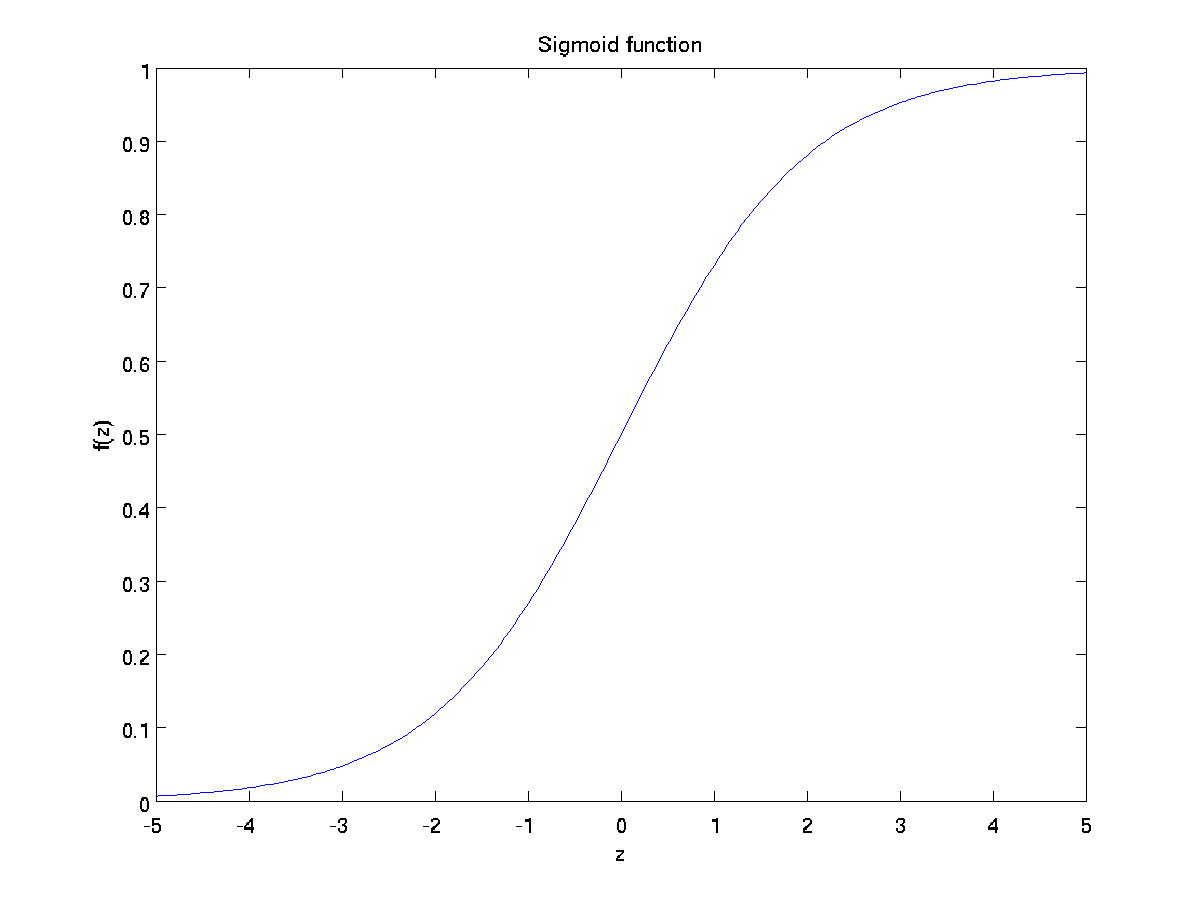
\includegraphics[width=0.45\textwidth]{figures/Sigmoid_Function.png}
%  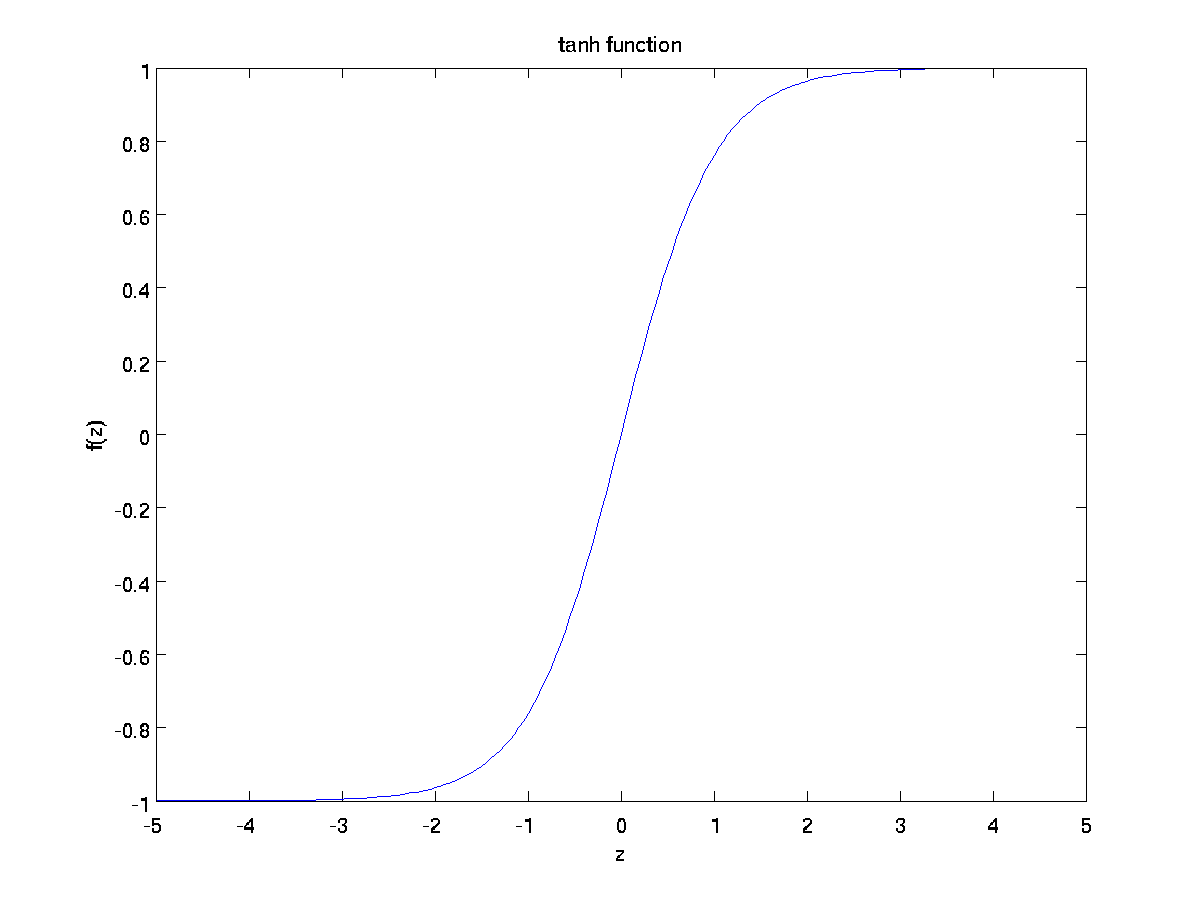
\includegraphics[width=0.45\textwidth]{figures/Tanh_Function.png}
%  %\caption{}\label{fig:step1}
%\end{figure}

\cnt{The $\tanh(z)$ function is a rescaled version of the sigmoid, and its output range is $[ -1,1]$ instead of $[0,1]$.}
    {$\tanh(z)$ 函数是sigmoid函数的一种变体,它的取值范围为 $[-1,1]$,而不是sigmoid函数的 $[0,1]$。}
    {}


\cnt{Note that unlike some other venues (including the OpenClassroom videos, and parts of CS229), we are not using the convention here of $x_0=1$. Instead, the intercept term is handled separately by the parameter $b$.}
    {注意,与其它地方(包括OpenClassroom公开课以及斯坦福大学CS229课程)不同的是,这里我们不再令 $x_0=1$。取而代之,我们用单独的参数 $b$ 来表示截距。}
    {}

\cnt{Finally, one identity that'll be useful later: If $f(z) = 1/(1+\exp(-z))$ is the sigmoid function, then its derivative is given by $f'(z) = f(z) (1-f(z))$. (If $f$ is the $\tanh$ function, then its derivative is given by $f'(z) = 1- (f(z))^2$.) You can derive this yourself using the definition of the sigmoid (or tanh) function.}
    {最后要说明的是,有一个等式我们以后会经常用到:如果选择 $f(z) = 1/(1+\exp(-z))$,也就是sigmoid函数,那么它的导数就是 $f'(z) = f(z) (1-f(z))$ (如果选择 $\tanh$ 函数,那它的导数就是 $f'(z) = 1- (f(z))^2$,你可以根据sigmoid(或tanh)函数的定义自行推导这个等式。}
    {}

\subsubsection{\cnt{Neural Network model}{神经网络模型}{}}

\cnt{A neural network\index{neural network} is put together by hooking together many of our simple ``neurons," so that the output of a neuron can be the input of another. For example, here is a small neural network:}
    {所谓 神经网络\index{神经网络} 就是将许多个单一“神经元”联结在一起,这样,一个“神经元”的输出就可以是另一个“神经元”的输入。例如,下图就是一个简单的神经网络:}
    {}

\begin{figure}[ht] \centering
  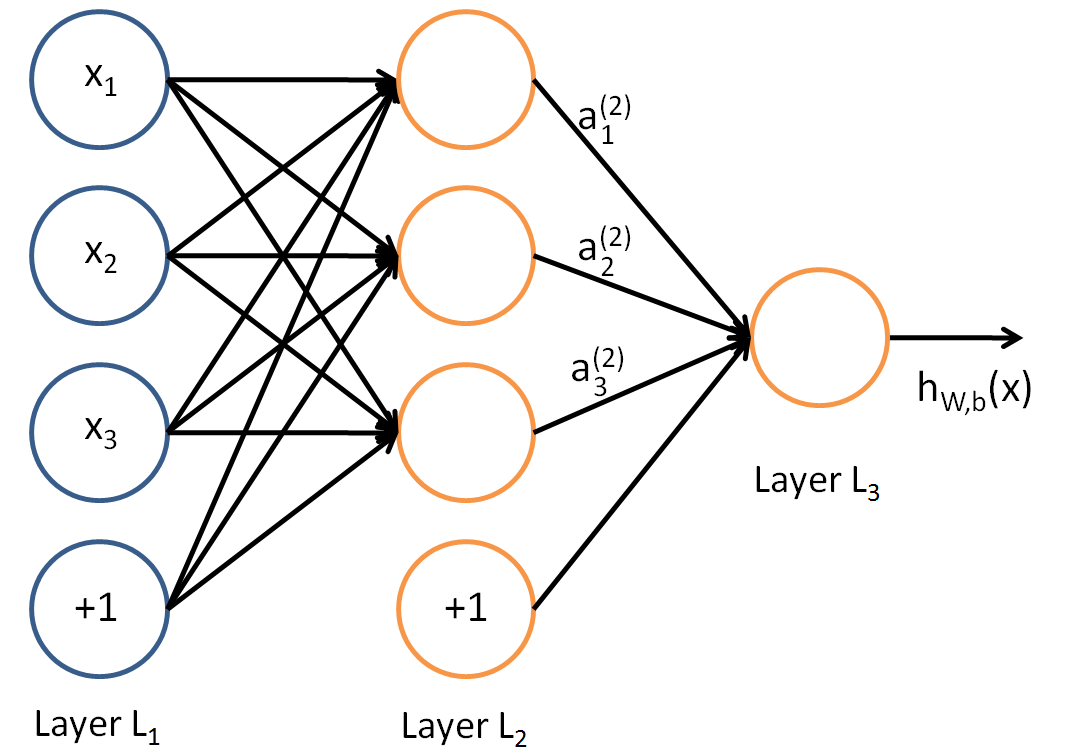
\includegraphics[width=0.6\textwidth]{figures/Network331.png}
  %\caption{}\label{fig:step1}
\end{figure}


\cnt{In this figure, we have used circles to also denote the inputs to the network. The circles labeled ``$+1$" are called \emph{bias units}, and correspond to the intercept term. The leftmost layer of the network is called the \emph{input layer}, and the rightmost layer the \emph{output layer} (which, in this example, has only one node). The middle layer of nodes is called the \emph{hidden layer}, because its values are not observed in the training set. We also say that our example neural network has 3 \emph{input units} (not counting the bias unit), 3 \emph{hidden units}, and 1 \emph{output unit}.}
    {我们使用圆圈来表示神经网络的输入,标上“$+1$”的圆圈被称为\emph{偏置节点},也就是截距项。神经网络最左边的一层叫做\emph{输入层},最右的一层叫做\emph{输出层}(本例中,输出层只有一个节点)。中间所有节点组成的一层叫做\emph{隐藏层},因为我们不能在训练样本集中观测到它们的值。同时可以看到,以上神经网络的例子中有3个输入单元(偏置单元不计在内),3个隐藏单元及一个输出单元。}
    {}


\cnt{We will let ${n}_l$ denote the number of layers in our network; thus $n_l=3$ in our example. We label layer $l$ as $L_l$, so layer $L_1$ is the input layer, and layer $L_{n_l}$ the output layer. Our neural network has parameters $(W,b) = (W^{(1)}, b^{(1)}, W^{(2)}, b^{(2)})$, where we write $W^{(l)}_{ij}$ to denote the parameter (or weight) associated with the connection between unit $j$ in layer $l$, and unit $i$ in layer $l + 1$. (Note the order of the indices.) Also, $b^{(l)}_i$ is the bias associated with unit $i$ in layer $l + 1$. Thus, in our example, we have $W^{(1)} \in \Re^{3\times 3}$, and $W^{(2)} \in \Re^{1\times 3}$. Note that bias units don't have inputs or connections going into them, since they always output the value $+1$. We also let $s_l$ denote the number of nodes in layer $l$ (not counting the bias unit).}
    {我们用 ${n}_l$ 来表示网络的层数,本例中 $n_l=3$,我们将第 $l$ 层记为 $L_l$,于是 $L_1$ 是输入层,输出层是 $L_{n_l}$。本例神经网络有参数 $(W,b) = (W^{(1)}, b^{(1)}, W^{(2)}, b^{(2)})$,其中 $W^{(l)}_{ij}$(下面的式子中用到)是第 $l$ 层第 $j$ 单元与第 $l+1$ 层第 $i$ 单元之间的联接参数(其实就是连接线上的权重,注意标号顺序), $b^{(l)}_i$ 是第 $l+1$ 层第 $i$ 单元的偏置项。因此在本例中, $W^{(1)} \in \Re^{3\times 3}$, $W^{(2)} \in \Re^{1\times 3}$。注意,没有其他单元连向偏置单元(即偏置单元没有输入),因为它们总是输出 $+1$。同时,我们用 $s_l$ 表示第 $l$ 层的节点数(偏置单元不计在内)。}
    {}

\cnt{We will write $a^{(l)}_i$ to denote the \emph{activation} (meaning output value) of unit $i$ in layer $l$. For $l = 1$, we also use $a^{(1)}_i = x_i$ to denote the $i$-th input. Given a fixed setting of the parameters $W,b$, our neural network defines a hypothesis $h_{W,b}(x)$ that outputs a real number. Specifically, the computation that this neural network represents is given by:}
    {我们用 $a^{(l)}_i$ 表示第 $l$ 层第 $i$ 单元的激活值(输出值)。当 $l=1$ 时, $a^{(1)}_i = x_i$,也就是第 $i$ 个输入值(输入值的第 $i$ 个特征)。对于给定参数集合 $W,b$,我们的神经网络就可以按照函数 $h_{W,b}(x)$ 来计算输出结果。本例神经网络的计算步骤如下:}
    {}

\begin{align*}
a_1^{(2)} &= f(W_{11}^{(1)}x_1 + W_{12}^{(1)} x_2 + W_{13}^{(1)} x_3 + b_1^{(1)})  \\
a_2^{(2)} &= f(W_{21}^{(1)}x_1 + W_{22}^{(1)} x_2 + W_{23}^{(1)} x_3 + b_2^{(1)})  \\
a_3^{(2)} &= f(W_{31}^{(1)}x_1 + W_{32}^{(1)} x_2 + W_{33}^{(1)} x_3 + b_3^{(1)})  \\
h_{W,b}(x) &= a_1^{(3)} =  f(W_{11}^{(2)}a_1^{(2)} + W_{12}^{(2)} a_2^{(2)} + W_{13}^{(2)} a_3^{(2)} + b_1^{(2)}) 
\end{align*}

\cnt{In the sequel, we also let $z^{(l)}_i$ denote the total weighted sum of inputs to unit $i$ in layer $l$, including the bias term (e.g., $z_i^{(2)} = \sum_{j=1}^n W^{(1)}_{ij} x_j + b^{(1)}_i)$, so that $a^{(l)}_i = f(z^{(l)}_i)$.}
    {我们用 $z^{(l)}_i$ 表示第 $l$ 层第 $i$ 单元输入加权和(包括偏置单元),比如, $z_i^{(2)} = \sum_{j=1}^n W^{(1)}_{ij} x_j + b^{(1)}_i$,则 $a^{(l)}_i = f(z^{(l)}_i)$。}
    {}


\cnt{Note that this easily lends itself to a more compact notation. Specifically, if we extend the activation function $f(\cdot)$ to apply to vectors in an element-wise fashion (i.e., $f([z_1, z_2, z_3]) = [f(z_1), f(z_2), f(z_3)]$, then we can write the equations above more compactly as:}
    {这样我们就可以得到一种更简洁的表示法。这里我们将激活函数 $f(\cdot)$ 扩展为用向量(分量的形式)来表示,即 $f([z_1, z_2, z_3]) = [f(z_1), f(z_2), f(z_3)]$,那么,上面的等式可以更简洁地表示为:}
    {}

\begin{align*}
z^{(2)} &= W^{(1)} x + b^{(1)} \\
a^{(2)} &= f(z^{(2)}) \\
z^{(3)} &= W^{(2)} a^{(2)} + b^{(2)} \\
h_{W,b}(x) &= a^{(3)} = f(z^{(3)})
\end{align*}

\cnt{We call this step \emph{forward propagation}\index{forward propagation}. More generally, recalling that we also use $a^{(1)} = x$ to also denote the values from the input layer, then given layer $l$'s activations $a^{(l)}$, we can compute layer $l + 1$'s activations $a^{(l+1)}$ as:}
    {我们将上面的计算步骤叫作\emph{前向传播}\index{前向传播}。回想一下,之前我们用 $a^{(1)} = x$ 表示输入层的激活值,那么给定第 $l$ 层的激活值 $a^{(l)}$ 后,第 $l+1$ 层的激活值 $a^{(l+1)}$ 就可以按照下面步骤计算得到:}
    {}

\begin{align*}
z^{(l+1)} &= W^{(l)} a^{(l)} + b^{(l)}   \\
a^{(l+1)} &= f(z^{(l+1)})
\end{align*}

\cnt{By organizing our parameters in matrices and using matrix-vector operations, we can take advantage of fast linear algebra routines to quickly perform calculations in our network.}
    {将参数矩阵化,使用矩阵-向量运算方式,我们就可以利用线性代数的优势对神经网络进行快速求解。}
    {}


\cnt{We have so far focused on one example neural network, but one can also build neural networks with other architectures (meaning patterns of connectivity between neurons), including ones with multiple hidden layers. The most common choice is a $n_l$-layered network where layer $1$ is the input layer, layer $n_l$ is the output layer, and each layer $l$ is densely connected to layer $l+1$. In this setting, to compute the output of the network, we can successively compute all the activations in layer $L_2$, then layer $L_3$, and so on, up to layer $L_{n_l}$, using the equations above that describe the forward propagation step. This is one example of a feedforward neural network, since the connectivity graph does not have any directed loops or cycles.}
    {目前为止,我们讨论了一种神经网络,我们也可以构建另一种结构的神经网络(这里结构指的是神经元之间的联接模式),也就是包含多个隐藏层的神经网络。最常见的一个例子是 $n_l$ 层的神经网络,第 $1$ 层是输入层,第 $n_l$ 层是输出层,中间的每个层 $l$ 与层 $l+1$ 紧密相联。这种模式下,要计算神经网络的输出结果,我们可以按照之前描述的等式,按部就班,进行前向传播,逐一计算第 $L_2$ 层的所有激活值,然后是第 $L_3$ 层的激活值,以此类推,直到第 $L_{n_l}$ 层。这是一个前馈神经网络的例子,因为这种联接图没有闭环或回路。}
    {}


\cnt{Neural networks can also have multiple output units. For example, here is a network with two hidden layers layers $L_2$ and $L_3$ and two output units in layer $L_4$:}
    {神经网络也可以有多个输出单元。比如,下面的神经网络有两层隐藏层: $L_2$ 及 $L_3$,输出层 $L_4$ 有两个输出单元。}
    {}

\begin{figure}[ht] \centering
  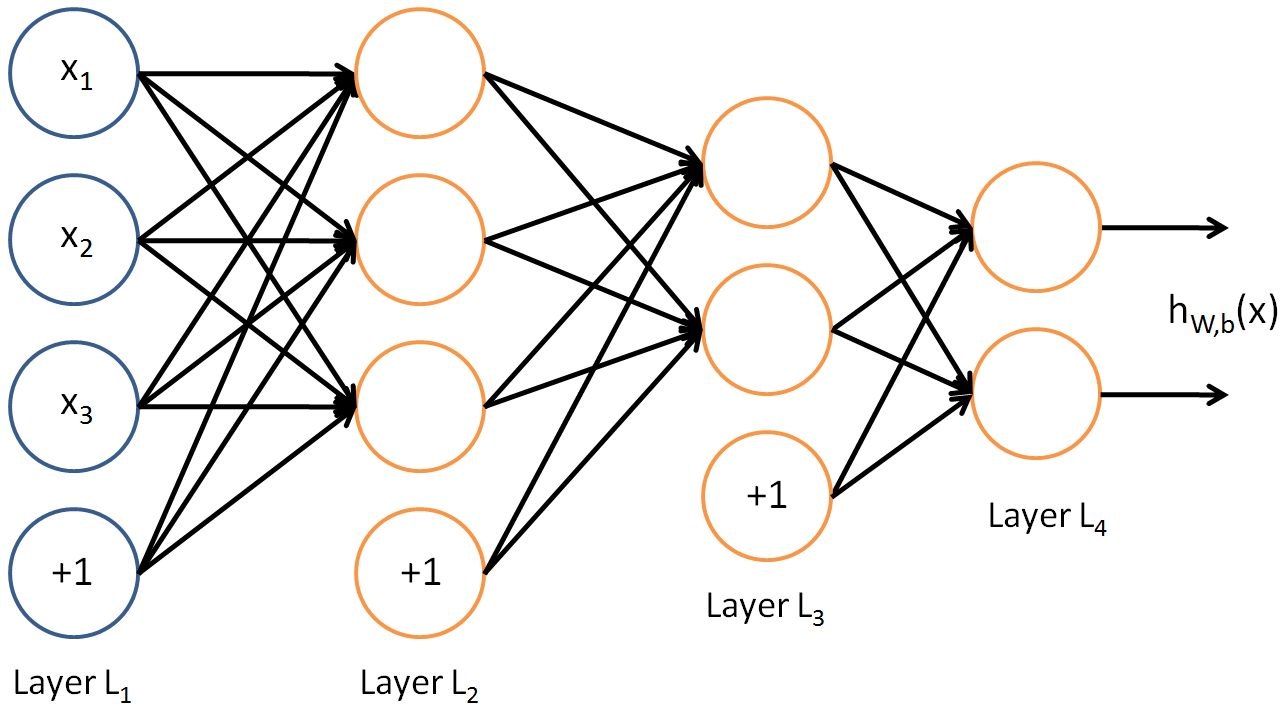
\includegraphics[width=0.7\textwidth]{figures/Network3322.png}
  %\caption{}\label{fig:step1}
\end{figure}

\cnt{To train this network, we would need training examples $(x^{(i)}, y^{(i)})$ where $y^{(i)} \in \Re^2$. This sort of network is useful if there're multiple outputs that you're interested in predicting. (For example, in a medical diagnosis application, the vector $x$ might give the input features of a patient, and the different outputs $y_i$'s might indicate presence or absence of different diseases.)}
    {要求解这样的神经网络,需要样本集 $(x^{(i)}, y^{(i)})$,其中 $y^{(i)} \in \Re^2$。如果你想预测的输出是多个的,那这种神经网络很适用。(比如,在医疗诊断应用中,患者的体征指标就可以作为向量$x$的输入值,而不同的输出值 $y_i$ 可以表示不同的疾病存在与否。)}
    {}


\subsection{\cnt{Backpropagation Algorithm}{反向传导算法}{}} \label{chp:bkpropgationalg}

\cnt{\index{backpropagation}}{\index{反向传导}}{}

\cnt{Suppose we have a fixed training set $\{ (x^{(1)}, y^{(1)}), \ldots, (x^{(m)}, y^{(m)}) \}$ of $m$ training examples. We can train our neural network using batch gradient descent. In detail, for a single training example $(x,y)$, we define the cost function with respect to that single example to be:
}
    {假设我们有一个固定样本集 $\{ (x^{(1)}, y^{(1)}), \ldots, (x^{(m)}, y^{(m)}) \}$,它包含 $m$ 个样例。我们可以用批量梯度下降法来求解神经网络。具体来讲,对于单个样例 $(x,y)$,其代价函数为:}
    {}


\begin{align}
J(W,b; x,y) = \frac{1}{2} \left\| h_{W,b}(x) - y \right\|^2.
\end{align}


\cnt{This is a (one-half) squared-error cost function. Given a training set of $m$ examples, we then define the overall cost function to be:}
    {这是一个(二分之一的)方差代价函数。给定一个包含 $m$ 个样例的数据集,我们可以定义整体代价函数为:}
    {}

 
\begin{align}
J(W,b)
&= \left[ \frac{1}{m} \sum_{i=1}^m J(W,b;x^{(i)},y^{(i)}) \right]
                       + \frac{\lambda}{2} \sum_{l=1}^{n_l-1} \; \sum_{i=1}^{s_l} \; \sum_{j=1}^{s_{l+1}} \left( W^{(l)}_{ji} \right)^2
 \\
&= \left[ \frac{1}{m} \sum_{i=1}^m \left( \frac{1}{2} \left\| h_{W,b}(x^{(i)}) - y^{(i)} \right\|^2 \right) \right]
                       + \frac{\lambda}{2} \sum_{l=1}^{n_l-1} \; \sum_{i=1}^{s_l} \; \sum_{j=1}^{s_{l+1}} \left( W^{(l)}_{ji} \right)^2
\end{align}


\cnt{The first term in the definition of J(W,b) is an average sum-of-squares error term. The second term is a regularization term (also called a \emph{weight decay} term) that tends to decrease the magnitude of the weights, and helps prevent overfitting.}
    {以上公式中的第一项 $J(W,b)$ 是一个均方差项。第二项是一个规则化项(也叫\emph{权重衰减项}),其目的是减小权重的幅度,防止过度拟合。}
    {}
\footnote{\cnt{Usually weight decay is not applied to the bias terms $b^{(l)}_i$, as reflected in our definition for $J(W,b)$. Applying weight decay to the bias units usually makes only a small difference to the final network, however. If you've taken CS229 (Machine Learning) at Stanford or watched the course's videos on YouTube, you may also recognize this weight decay as essentially a variant of the Bayesian regularization method you saw there, where we placed a Gaussian prior on the parameters and did MAP (instead of maximum likelihood) estimation.}{通常权重衰减的计算并不使用偏置项 $b^{(l)}_i$,比如我们在 $J(W, b)$ 的定义中就没有使用。一般来说,将偏置项包含在权重衰减项中只会对最终的神经网络产生很小的影响。如果你在斯坦福选修过CS229(机器学习)课程,或者在YouTube上看过课程视频,你会发现这个权重衰减实际上是课上提到的贝叶斯规则化方法的变种。在贝叶斯规则化方法中,我们将高斯先验概率引入到参数中计算MAP(极大后验)估计(而不是极大似然估计)。}{}}

\cnt{The \emph{weight decay parameter} $\lambda$ controls the relative importance of the two terms. Note also the slightly overloaded notation: $J(W,b;x,y)$ is the squared error cost with respect to a single example; $J(W,b)$ is the overall cost function, which includes the weight decay term.}
    {\emph{权重衰减参数} $\lambda$ 用于控制公式中两项的相对重要性。在此重申一下这两个复杂函数的含义:$J(W,b;x,y)$ 是针对单个样例计算得到的方差代价函数;$J(W,b)$ 是整体样本代价函数,它包含权重衰减项。}
    {}


\cnt{This cost function above is often used both for classification and for regression problems. For classification, we let $y = 0$ or $1$ represent the two class labels (recall that the sigmoid activation function outputs values in $[0,1]$; if we were using a tanh activation function, we would instead use $-1$ and $+1$ to denote the labels). For regression problems, we first scale our outputs to ensure that they lie in the $[0,1]$ range (or if we were using a tanh activation function, then the $[-1,1]$ range).}
    {以上的代价函数经常被用于分类和回归问题。在分类问题中,我们用 $y = 0$ 或 $1$,来代表两种类型的标签(回想一下,这是因为 sigmoid激活函数的值域为 $[0,1]$;如果我们使用双曲正切型激活函数,那么应该选用 $-1$ 和 $+1$ 作为标签)。对于回归问题,我们首先要变换输出值域(译者注:也就是 $y$),以保证其范围为 $[0,1]$ (同样地,如果我们使用双曲正切型激活函数,要使输出值域为 $[-1,1]$)。}
    {}

\cnt{Our goal is to minimize $J(W,b)$ as a function of $W$ and $b$. To train our neural network, we will initialize each parameter $W^{(l)}_{ij}$ and each $b^{(l)}_i$ to a small random value near zero (say according to a ${Normal}(0,\epsilon^2)$ distribution for some small $\epsilon$, say $0.01$), and then apply an optimization algorithm such as batch gradient descent. Since $J(W,b)$ is a non-convex function, gradient descent is susceptible to local optima; however, in practice gradient descent usually works fairly well. Finally, note that it is important to initialize the parameters randomly, rather than to all $0$'s. If all the parameters start off at identical values, then all the hidden layer units will end up learning the same function of the input (more formally, $W^{(1)}_{ij}$ will be the same for all values of $i$, so that $a^{(2)}_1 = a^{(2)}_2 = a^{(2)}_3 = \ldots$ for any input $x$). The random initialization serves the purpose of \emph{symmetry breaking}.}
    {我们的目标是针对参数 $W$ 和 $b$ 来求其函数 $J(W,b)$ 的最小值。为了求解神经网络,我们需要将每一个参数 $W^{(l)}_{ij}$ 和 $b^{(l)}_i$ 初始化为一个很小的、接近零的随机值(比如说,使用正态分布 ${Normal}(0,\epsilon^2)$ 生成的随机值,其中 $\epsilon$ 设置为 $0.01$ ),之后对目标函数使用诸如批量梯度下降法的最优化算法。因为 $J(W, b)$ 是一个非凸函数,梯度下降法很可能会收敛到局部最优解;但是在实际应用中,梯度下降法通常能得到令人满意的结果。最后,需要再次强调的是,要将参数进行随机初始化,而不是全部置为 $0$。如果所有参数都用相同的值作为初始值,那么所有隐藏层单元最终会得到与输入值有关的、相同的函数(也就是说,对于所有 $i$,$W^{(1)}_{ij}$ 都会取相同的值,那么对于任何输入 $x$ 都会有:$a^{(2)}_1 = a^{(2)}_2 = a^{(2)}_3 = \ldots$ )。随机初始化的目的是使\emph{对称失效}。}
    {}


\cnt{One iteration of gradient descent updates the parameters $W,b$ as follows:}
    {梯度下降法中每一次迭代都按照如下公式对参数 $W$ 和 $b$ 进行更新:}
    {}

\begin{align}
W_{ij}^{(l)} &= W_{ij}^{(l)} - \alpha \frac{\partial}{\partial W_{ij}^{(l)}} J(W,b) \\
b_{i}^{(l)} &= b_{i}^{(l)} - \alpha \frac{\partial}{\partial b_{i}^{(l)}} J(W,b)
\end{align}


\cnt{where $\alpha$ is the learning rate. The key step is computing the partial derivatives above. We will now describe the \emph{backpropagation algorithm}, which gives an efficient way to compute these partial derivatives.}
    {其中 $\alpha$ 是学习速率。其中关键步骤是计算偏导数。我们现在来讲一下\emph{反向传播算法},它是计算偏导数的一种有效方法。}
    {}


\cnt{We will first describe how backpropagation can be used to compute $\frac{\partial}{\partial W_{ij}^{(l)}} J(W,b; x, y)$ and $\frac{\partial}{\partial b_{i}^{(l)}} J(W,b; x, y)$, the partial derivatives of the cost function $J(W,b;x,y)$ defined with respect to a single example $(x,y)$. Once we can compute these, we see that the derivative of the overall cost function $J(W,b)$ can be computed as:}
    {我们首先来讲一下如何使用反向传播算法来计算 $\frac{\partial}{\partial W_{ij}^{(l)}} J(W,b; x, y)$ 和 $\frac{\partial}{\partial b_{i}^{(l)}} J(W,b; x, y)$,这两项是单个样例 $(x,y)$ 的代价函数 $J(W,b;x,y)$ 的偏导数。一旦我们求出该偏导数,就可以推导出整体代价函数 $J(W,b)$ 的偏导数:}
    {}


\begin{align}
\frac{\partial}{\partial W_{ij}^{(l)}} J(W,b) &=
\left[ \frac{1}{m} \sum_{i=1}^m \frac{\partial}{\partial W_{ij}^{(l)}} J(W,b; x^{(i)}, y^{(i)}) \right] + \lambda W_{ij}^{(l)} \\
\frac{\partial}{\partial b_{i}^{(l)}} J(W,b) &=
\frac{1}{m}\sum_{i=1}^m \frac{\partial}{\partial b_{i}^{(l)}} J(W,b; x^{(i)}, y^{(i)})
\end{align}

\cnt{The two lines above differ slightly because weight decay is applied to $W$ but not $b$.}
    {以上两行公式稍有不同,第一行比第二行多出一项,是因为权重衰减是作用于 $W$ 而不是 $b$。}
    {}


\cnt{The intuition behind the backpropagation algorithm is as follows. Given a training example $(x,y)$, we will first run a ``forward pass" to compute all the activations throughout the network, including the output value of the hypothesis $h_{W,b}(x)$. Then, for each node $i$ in layer $l$, we would like to compute an ``error term" $\delta^{(l)}_i$ that measures how much that node was ``responsible" for any errors in our output. For an output node, we can directly measure the difference between the network's activation and the true target value, and use that to define $\delta^{(n_l)}_i$ (where layer $n_l$ is the output layer). How about hidden units? For those, we will compute $\delta^{(l)}_i$ based on a weighted average of the error terms of the nodes that uses $a^{(l)}_i$ as an input. In detail, here is the backpropagation algorithm:}
    {反向传播算法的思路如下:给定一个样例 $(x,y)$,我们首先进行“前向传导”运算,计算出网络中所有的激活值,包括 $h_{W,b}(x)$ 的输出值。之后,针对第 $l$ 层的每一个节点 $i$,我们计算出其“残差” $\delta^{(l)}_i$,该残差表明了该节点对最终输出值的残差产生了多少影响。对于最终的输出节点,我们可以直接算出网络产生的激活值与实际值之间的差距,我们将这个差距定义为 $\delta^{(n_l)}_i$ (第 $n_l$ 层表示输出层)。对于隐藏单元我们如何处理呢?我们将基于节点(译者注:第 $l+1$ 层节点)残差的加权平均值计算 $\delta^{(l)}_i$,这些节点以 $a^{(l)}_i$ 作为输入。下面将给出反向传导算法的细节:}
    {}

\begin{enumerate}
  \item
\cnt{Perform a feedforward pass, computing the activations for layers $L_2, L_3, \ldots$, and so on up to the output layer $L_{n_l}$.}
    {进行前馈传导计算,利用前向传导公式,得到 $L_2, L_3, \ldots$ 直到输出层 $L_{n_l}$ 的激活值。}
    {}

  \item
\cnt{For each output unit $i$ in layer $n_l$ (the output layer), set}
    {对于第 $n_l$ 层(输出层)的每个输出单元 $i$,我们根据以下公式计算残差:}
    {}

\begin{align}
\delta^{(n_l)}_i
= \frac{\partial}{\partial z^{(n_l)}_i} \;\;
        \frac{1}{2} \left\|y - h_{W,b}(x)\right\|^2 = - (y_i - a^{(n_l)}_i) \cdot f'(z^{(n_l)}_i)
\end{align}
\footnote{译者注:

\begin{align}
\delta^{(n_l)}_i &= \frac{\partial}{\partial z^{n_l}_i}J(W,b;x,y)
 = \frac{\partial}{\partial z^{n_l}_i}\frac{1}{2} \left\|y - h_{W,b}(x)\right\|^2 \\
 &= \frac{\partial}{\partial z^{n_l}_i}\frac{1}{2} \sum_{j=1}^{S_{n_l}} (y_j-a_j^{(n_l)})^2
 = \frac{\partial}{\partial z^{n_l}_i}\frac{1}{2} \sum_{j=1}^{S_{n_l}} (y_j-f(z_j^{(n_l)}))^2 \\
 &= - (y_i - f(z_i^{(n_l)})) \cdot f'(z^{(n_l)}_i)
 = - (y_i - a^{(n_l)}_i) \cdot f'(z^{(n_l)}_i)
\end{align}
}

  \item
\cnt{For $l = n_l-1, n_l-2, n_l-3, \ldots, 2$}
    {对 $l = n_l-1, n_l-2, n_l-3, \ldots, 2$ 的各个层,}
    {}

\cnt{For each node $i$ in layer $l$, set}
    {计算第 $l$ 层的第 $i$ 个节点的残差:}
    {}
$$
\delta^{(l)}_i = \left( \sum_{j=1}^{s_{l+1}} W^{(l)}_{ji} \delta^{(l+1)}_j \right) f'(z^{(l)}_i)
$$
\footnote{译者注:
 
\begin{align}
\delta^{(n_l-1)}_i &=\frac{\partial}{\partial z^{n_l-1}_i}J(W,b;x,y)
 = \frac{\partial}{\partial z^{n_l-1}_i}\frac{1}{2} \left\|y - h_{W,b}(x)\right\|^2 
 = \frac{\partial}{\partial z^{n_l-1}_i}\frac{1}{2} \sum_{j=1}^{S_{n_l}}(y_j-a_j^{(n_l)})^2 \\
&= \frac{1}{2} \sum_{j=1}^{S_{n_l}}\frac{\partial}{\partial z^{n_l-1}_i}(y_j-a_j^{(n_l)})^2
 = \frac{1}{2} \sum_{j=1}^{S_{n_l}}\frac{\partial}{\partial z^{n_l-1}_i}(y_j-f(z_j^{(n_l)}))^2 \\
&= \sum_{j=1}^{S_{n_l}}-(y_j-f(z_j^{(n_l)})) \cdot \frac{\partial}{\partial z_i^{(n_l-1)}}f(z_j^{(n_l)})
 = \sum_{j=1}^{S_{n_l}}-(y_j-f(z_j^{(n_l)})) \cdot  f'(z_j^{(n_l)}) \cdot \frac{\partial z_j^{(n_l)}}{\partial z_i^{(n_l-1)}} \\
&= \sum_{j=1}^{S_{n_l}} \delta_j^{(n_l)} \cdot \frac{\partial z_j^{(n_l)}}{\partial z_i^{n_l-1}}
 = \sum_{j=1}^{S_{n_l}} \left(\delta_j^{(n_l)} \cdot \frac{\partial}{\partial z_i^{n_l-1}}\sum_{k=1}^{S_{n_l-1}}f(z_k^{n_l-1}) \cdot W_{jk}^{n_l-1}\right) \\
&= \sum_{j=1}^{S_{n_l}} \delta_j^{(n_l)} \cdot  W_{ji}^{n_l-1} \cdot f'(z_i^{n_l-1})
 = \left(\sum_{j=1}^{S_{n_l}}W_{ji}^{n_l-1}\delta_j^{(n_l)}\right)f'(z_i^{n_l-1})
\end{align}

将上式中的 $n_l-1$ 与 $n_l$ 的关系替换为 $l$ 与 $l+1$ 的关系,就可以得到:
$$\delta^{(l)}_i = \left( \sum_{j=1}^{s_{l+1}} W^{(l)}_{ji} \delta^{(l+1)}_j \right) f'(z^{(l)}_i)$$
以上逐次从后向前求导的过程即为“反向传导”的本意所在。
}

  \item
\cnt{Compute the desired partial derivatives, which are given as:}
    {计算我们需要的偏导数,计算方法如下:}
    {}

\begin{align}
\frac{\partial}{\partial W_{ij}^{(l)}} J(W,b; x, y) &= a^{(l)}_j \delta_i^{(l+1)} \\
\frac{\partial}{\partial b_{i}^{(l)}} J(W,b; x, y) &= \delta_i^{(l+1)}.
\end{align}

\end{enumerate}

\cnt{Finally, we can also re-write the algorithm using matrix-vectorial notation. We will use ``$\bullet$" to denote the element-wise product operator (denoted ``\texttt{.*}" in Matlab or Octave, and also called the Hadamard product), so that if $a = b \bullet c$, then $a_i = b_ic_i$. Similar to how we extended the definition of $f(\cdot)$ to apply element-wise to vectors, we also do the same for $f'(\cdot)$ (so that $f'([z_1, z_2, z_3]) =[f'(z_1),f'(z_2),f'(z_3)]$ ).}
    {最后,我们用矩阵-向量表示法重写以上算法。我们使用“$\bullet$” 表示向量乘积运算符(在Matlab或Octave里用“\texttt{.*}”表示,也称作阿达马乘积)。若 $a = b \bullet c$,则 $a_i = b_ic_i$。在上一个教程中我们扩展了 $f(\cdot)$ 的定义,使其包含向量运算,这里我们也对偏导数 $f'(\cdot)$ 也做了同样的处理(于是又有  $f'([z_1, z_2, z_3]) = [f'(z_1), f'(z_2), f'(z_3)]$)。}
    {}


\cnt{The algorithm can then be written:}
    {那么,反向传播算法可表示为以下几个步骤:}
    {}

\begin{enumerate}
  \item
\cnt{Perform a feedforward pass, computing the activations for layers $L_2$, $L_3$, up to the output layer $L_{n_l}$, using the equations defining the forward propagation steps}
    {进行前馈传导计算,利用前向传导公式,得到 $L_2, L_3, \ldots$ 直到输出层 $L_{n_l}$ 的激活值。}
    {}

  \item
\cnt{For the output layer (layer $n_l$), set}
    {对输出层(第 $n_l$ 层),计算:}
    {}

\begin{align}
\delta^{(n_l)}
= - (y - a^{(n_l)}) \bullet f'(z^{(n_l)})
\end{align}

  \item
\cnt{For $l = n_l-1, n_l-2, n_l-3, \ldots, 2$, Set}
    {对于 $l = n_l-1, n_l-2, n_l-3, \ldots, 2$ 的各层,计算:}
    {}

\begin{align}
\delta^{(l)} = \left((W^{(l)})^T \delta^{(l+1)}\right) \bullet f'(z^{(l)})
\end{align}

  \item
\cnt{Compute the desired partial derivatives:}
    {计算最终需要的偏导数值:}
    {}

\begin{align}
\nabla_{W^{(l)}} J(W,b;x,y) &= \delta^{(l+1)} (a^{(l)})^T, \\
\nabla_{b^{(l)}} J(W,b;x,y) &= \delta^{(l+1)}.
\end{align}

\end{enumerate}

\cnt{\emph{Implementation note}: In steps 2 and 3 above, we need to compute $f'(z^{(l)}_i)$ for each value of $i$. Assuming $f(z)$ is the sigmoid activation function, we would already have $a^{(l)}_i$ stored away from the forward pass through the network. Thus, using the expression that we worked out earlier for $f'(z)$, we can compute this as $f'(z^{(l)}_i) = a^{(l)}_i (1- a^{(l)}_i)$.}
    {\emph{实现中应注意}:在以上的第2步和第3步中,我们需要为每一个 $i$ 值计算其 $f'(z^{(l)}_i$)。假设 $f(z)$ 是sigmoid函数,并且我们已经在前向传导运算中得到了 $a^{(l)}_i$。那么,使用我们早先推导出的 $f'(z)$ 表达式,就可以计算得到 $f'(z^{(l)}_i) = a^{(l)}_i (1- a^{(l)}_i)$。}
    {}

\cnt{Finally, we are ready to describe the full gradient descent algorithm. In the pseudo-code below, $\Delta W^{(l)}$ is a matrix (of the same dimension as $W^{(l)}$), and $\Delta b^{(l)}$ is a vector (of the same dimension as $b^{(l)}$). Note that in this notation, ``$\Delta W^{(l)}$" is a matrix, and in particular it isn't ``$\Delta$ times $W^{(l)}$." We implement one iteration of batch gradient descent as follows:}
    {最后,我们将对梯度下降算法做个全面总结。在下面的伪代码中,$\Delta W^{(l)}$ 是一个与矩阵 $W^{(l)}$ 维度相同的矩阵,$\Delta b^{(l)}$ 是一个与 $b^{(l)}$ 维度相同的向量。注意这里“$\Delta W^{(l)}$”是一个矩阵,而不是“$\Delta$ 与 $W^{(l)}$ 相乘”。下面,我们实现批量梯度下降法中的一次迭代:}
    {}

\begin{enumerate}
  \item
\cnt{Set $\Delta W^{(l)} := 0$, $\Delta b^{(l)} := 0$ (matrix/vector of zeros) for all $l$.}
    {对于所有 $l$,令 $\Delta W^{(l)} := 0$, $\Delta b^{(l)} := 0$ (设置为全零矩阵或全零向量)}
    {}

  \item
\cnt{or $i = 1$ to $m$,}
    {对于 $i = 1$ 到 $m$,}
    {}
    \begin{enumerate}
      \item
\cnt{Use backpropagation to compute $\nabla_{W^{(l)}} J(W,b;x,y)$ and $\nabla_{b^{(l)}} J(W,b;x,y)$.}
    {使用反向传播算法计算 $\nabla_{W^{(l)}} J(W,b;x,y)$ 和 $\nabla_{b^{(l)}} J(W,b;x,y)$。}
    {}
      \item
\cnt{Set $\Delta W^{(l)} := \Delta W^{(l)} + \nabla_{W^{(l)}} J(W,b;x,y)$.}
    {计算 $\Delta W^{(l)} := \Delta W^{(l)} + \nabla_{W^{(l)}} J(W,b;x,y)$。}
    {}
      \item
\cnt{Set $\Delta b^{(l)} := \Delta b^{(l)} + \nabla_{b^{(l)}} J(W,b;x,y)$.}
    {计算 $\Delta b^{(l)} := \Delta b^{(l)} + \nabla_{b^{(l)}} J(W,b;x,y)$。}
    {}
    \end{enumerate}

  \item
\cnt{Update the parameters:}
    {更新权重参数:}
    {}

 \begin{align}
W^{(l)} &= W^{(l)} - \alpha \left[ \left(\frac{1}{m} \Delta W^{(l)} \right) + \lambda W^{(l)}\right] \\
b^{(l)} &= b^{(l)} - \alpha \left[\frac{1}{m} \Delta b^{(l)}\right]
\end{align}

\end{enumerate}

\cnt{To train our neural network, we can now repeatedly take steps of gradient descent to reduce our cost function $J(W,b)$.}
    {现在,我们可以重复梯度下降法的迭代步骤来减小代价函数 $J(W,b)$ 的值,进而求解我们的神经网络。}
    {}


\subsection{\cnt{Gradient checking and advanced optimization}{梯度检验与高级优化}{}} \label{chp:gradcheckingopt}

\cnt{Backpropagation is a notoriously difficult algorithm to debug and get right, especially since many subtly buggy implementations of it -- for example, one that has an off-by-one error in the indices and that thus only trains some of the layers of weights, or an implementation that omits the bias term -- will manage to learn something that can look surprisingly reasonable (while performing less well than a correct implementation). Thus, even with a buggy implementation, it may not at all be apparent that anything is amiss. In this section, we describe a method for numerically checking the derivatives computed by your code to make sure that your implementation is correct. Carrying out the derivative checking procedure described here will significantly increase your confidence in the correctness of your code.}
    {众所周知,反向传播算法很难调试得到正确结果,尤其是当实现程序存在很多难于发现的bug时。举例来说,索引的缺位错误(off-by-one error)会导致只有部分层的权重得到训练,再比如忘记计算偏置项。这些错误会使你得到一个看似十分合理的结果(但实际上比正确代码的结果要差)。因此,但从计算结果上来看,我们很难发现代码中有什么东西遗漏了。本节中,我们将介绍一种对求导结果进行数值检验的方法,该方法可以验证求导代码是否正确。另外,使用本节所述求导检验方法,可以帮助你提升写正确代码的信心。}
    {}
\cnt{}
    {\footnote{缺位错误(Off-by-one error)举例说明:比如 $for$ 循环中循环 $m$ 次,正确应该是 $for (i=1;~i<=m;~i++)$,但有时程序员疏忽,会写成 $for (i=1;~i<m;~i++)$,这就是缺位错误。}}
    {}

\cnt{Suppose we want to minimize $J(\theta)$ as a function of $\theta$. For this example, suppose $J : \Re \mapsto \Re$, so that $\theta \in \Re$. In this 1-dimensional case, one iteration of gradient descent is given by}
    {假设我们想要最小化以 $\theta$ 为自变量的目标函数 $J(\theta)$。假设 $J : \Re \mapsto \Re$,则 $\theta \in \Re$。在一维的情况下,一次迭代的梯度下降公式是}
    {}

\begin{align}
\theta := \theta - \alpha \frac{d}{d\theta}J(\theta).
\end{align}

\cnt{Suppose also that we have implemented some function $g(\theta)$ that purportedly computes $\frac{d}{d\theta}J(\theta)$, so that we implement gradient descent using the update $\theta := \theta - \alpha g(\theta)$. How can we check if our implementation of $g$ is correct?}
    {再假设我们已经用代码实现了计算 $\frac{d}{d\theta}J(\theta)$ 的函数 $g(\theta)$,接着我们使用 $\theta := \theta - \alpha g(\theta)$ 来实现梯度下降算法。那么我们如何检验 $g$ 的实现是否正确呢?}
    {}

\cnt{Recall the mathematical definition of the derivative as}
    {回忆导数的数学定义:}
    {}

\begin{align}
\frac{d}{d\theta}J(\theta) = \lim_{\epsilon \rightarrow 0}
\frac{J(\theta+ \epsilon) - J(\theta-\epsilon)}{2 \epsilon}.
\end{align}

\cnt{Thus, at any specific value of $\theta$, we can numerically approximate the derivative as follows:}
    {那么对于任意 $\theta$ 值,我们都可以对等式左边的导数用:}
    {}

\begin{align}
\frac{J(\theta+{\rm EPSILON}) - J(\theta-{\rm EPSILON})}{2 \times {\rm EPSILON}}
\end{align}

\cnt{}
    {来近似。}
    {}


\cnt{In practice, we set EPSILON to a small constant, say around $10^{-4}$. (There's a large range of values of EPSILON that should work well, but we don't set EPSILON to be ``extremely" small, say $10^{-20}$, as that would lead to numerical roundoff errors.)}
    {实际应用中,我们常将 $EPSILON$ 设为一个很小的常量,比如在 $10^{-4}$ 数量级(虽然 $EPSILON$ 的取值范围可以很大,但是我们不会将它设得太小,比如 $10^{-20}$,因为那将导致数值舍入误差。)}
    {}

\cnt{Thus, given a function $g(\theta)$ that is supposedly computing $\frac{d}{d\theta}J(\theta)$, we can now numerically verify its correctness by checking that}
    {给定一个被认为能计算 $\frac{d}{d\theta}J(\theta)$ 的函数 $g(\theta)$,我们可以用下面的数值检验公式}
    {}

\begin{align}
g(\theta) \approx
\frac{J(\theta+{\rm EPSILON}) - J(\theta-{\rm EPSILON})}{2 \times {\rm EPSILON}}.
\end{align}

\cnt{}
    {计算两端是否一样来检验函数是否正确。}
    {}


\cnt{The degree to which these two values should approximate each other will depend on the details of $J$. But assuming ${\rm EPSILON} = 10^{-4}$, you'll usually find that the left- and right-hand sides of the above will agree to at least 4 significant digits (and often many more).}
    {上式两端值的接近程度取决于 $J$ 的具体形式。但是在假定 ${\rm EPSILON} = 10^{-4}$ 的情况下,你通常会发现上式左右两端至少有4位有效数字是一样的(通常会更多)。}
    {}


\cnt{Now, consider the case where $\theta \in \Re^n$ is a vector rather than a single real number (so that we have $n$ parameters that we want to learn), and $J: \Re^n \mapsto \Re$. In our neural network example we used ``$J(W,b)$," but one can imagine ``unrolling" the parameters $W,b$ into a long vector $\theta$. We now generalize our derivative checking procedure to the case where $\theta$ may be a vector.}
    {现在,考虑 $\theta \in \Re^n$ 是一个向量而非一个实数(那么就有 $n$ 个参数要学习得到),并且 $J: \Re^n \mapsto \Re$。在神经网络的例子里我们使用 $J(W,b)$,可以想象为把参数 $W,b$ 组合扩展成一个长向量 $\theta$。现在我们将求导检验方法推广到一般化,即 $\theta$ 是一个向量的情况。}
    {}

\cnt{Suppose we have a function $g_i(\theta)$ that purportedly computes $\frac{\partial}{\partial \theta_i} J(\theta)$; we'd like to check if $g_i$ is outputting correct derivative values. Let $\theta^{(i+)} = \theta + {\rm EPSILON} \times \vec{e}_i$, where}
    {假设我们有一个用于计算 $\frac{\partial}{\partial \theta_i} J(\theta)$ 的函数 $g_i(\theta)$;我们想要检验 $g_i$ 是否输出正确的求导结果。我们定义 $\theta^{(i+)} = \theta + {\rm EPSILON} \times \vec{e}_i$,其中}
    {}
\begin{align}
\vec{e}_i = \begin{bmatrix}0 \\ 0 \\ \vdots \\ 1 \\ \vdots \\ 0\end{bmatrix}
\end{align}
\cnt{is the $i$-th basis vector (a vector of the same dimension as $\theta$, with a ``1" in the $i$-th position and ``0"s everywhere else). So, $\theta^{(i+)}$ is the same as $\theta$, except its $i$-th element has been incremented by EPSILON. Similarly, let $\theta^{(i-)} = \theta - {\rm EPSILON} \times \vec{e}_i$ be the corresponding vector with the $i$-th element decreased by EPSILON. We can now numerically verify $g_i(\theta)$'s correctness by checking, for each $i$, that:}
    {是第 $i$ 个基向量(维度和 $\theta$ 相同,在第 $i$ 行是“$1$”而其他行是“$0$”)。所以,$\theta^{(i+)}$ 和 $\theta$ 几乎相同,除了第 $i$ 行元素增加了 $EPSILON$。类似地,$\theta^{(i-)} = \theta - {\rm EPSILON} \times \vec{e}_i$ 得到的第 $i$ 行减小了 $EPSILON$。然后我们可以对每个 $i$ 检查下式是否成立,进而验证 $g_i(\theta)$ 的正确性:}
    {}

\begin{align}
g_i(\theta) \approx
\frac{J(\theta^{(i+)}) - J(\theta^{(i-)})}{2 \times {\rm EPSILON}}.
\end{align}

\cnt{When implementing backpropagation to train a neural network, in a correct implementation we will have that}
    {当用反射传播算法求解神经网络时,正确算法实现会得到:}
    {}

\begin{align}
\nabla_{W^{(l)}} J(W,b) &= \left( \frac{1}{m} \Delta W^{(l)} \right) + \lambda W^{(l)} \\
\nabla_{b^{(l)}} J(W,b) &= \frac{1}{m} \Delta b^{(l)}.
\end{align}

\cnt{This result shows that the final block of psuedo-code in Backpropagation Algorithm \ref{chp:bkpropgationalg} is indeed implementing gradient descent. To make sure your implementation of gradient descent is correct, it is usually very helpful to use the method described above to numerically compute the derivatives of $J(W,b)$, and thereby verify that your computations of $\left(\frac{1}{m}\Delta W^{(l)} \right) + \lambda W$ and $\frac{1}{m}\Delta b^{(l)}$ are indeed giving the derivatives you want.}
    {以上结果与反向传播算法(\ref{chp:bkpropgationalg})中的最后一段伪代码一致,都是计算梯度下降。为了验证梯度下降代码的正确性,使用上述数值检验方法计算 $J(W,b)$ 的导数,然后验证 $\left(\frac{1}{m}\Delta W^{(l)} \right) + \lambda W$ 与 $\frac{1}{m}\Delta b^{(l)}$ 是否能够给出正确的求导结果。}
    {}

\cnt{Finally, so far our discussion has centered on using gradient descent to minimize $J(\theta)$. If you have implemented a function that computes $J(\theta)$ and $\nabla_\theta J(\theta)$, it turns out there are more sophisticated algorithms than gradient descent for trying to minimize $J(\theta)$. For example, one can envision an algorithm that uses gradient descent, but automatically tunes the learning rate $\alpha$ so as to try to use a step-size that causes $\theta$ to approach a local optimum as quickly as possible. There are other algorithms that are even more sophisticated than this; for example, there are algorithms that try to find an approximation to the Hessian matrix, so that it can take more rapid steps towards a local optimum (similar to Newton's method). A full discussion of these algorithms is beyond the scope of these notes, but one example is the L-BFGS algorithm. (Another example is the conjugate gradient algorithm.) You will use one of these algorithms in the programming exercise. The main thing you need to provide to these advanced optimization algorithms is that for any $\theta$, you have to be able to compute $J(\theta)$ and $\nabla_\theta J(\theta)$. These optimization algorithms will then do their own internal tuning of the learning rate/step-size $\alpha$ (and compute its own approximation to the Hessian, etc.) to automatically search for a value of $\theta$ that minimizes $J(\theta)$. Algorithms such as L-BFGS and conjugate gradient can often be much faster than gradient descent.}
    {迄今为止,我们的讨论都集中在使用梯度下降法来最小化 $J(\theta)$。如果你已经实现了一个计算 $J(\theta)$ 和 $\nabla_\theta J(\theta)$ 的函数,那么其实还有更精妙的算法来最小化 $J(\theta)$。举例来说,可以想象这样一个算法:它使用梯度下降,并能够自动调整学习速率 $\alpha$,以得到合适的步长值,最终使 $\theta$ 能够快速收敛到一个局部最优解。还有更妙的算法:比如可以寻找一个Hessian矩阵的近似,得到最佳步长值,使用该步长值能够更快地收敛到局部最优(和牛顿法类似)。此类算法的详细讨论已超出了这份讲义的范围,但是L-BFGS算法我们以后会有论述(另一个例子是共轭梯度算法)。你将在编程练习里使用这些算法中的一个。使用这些高级优化算法时,你需要提供关键的函数:即对于任一个 $\theta$,需要你计算出 $J(\theta)$ 和 $\nabla_\theta J(\theta)$。之后,这些优化算法会自动调整学习速率/步长值 $\alpha$ 的大小(并计算Hessian近似矩阵等等)来自动寻找 $J(\theta)$ 最小化时 $\theta$ 的值。诸如L-BFGS和共轭梯度算法通常比梯度下降法快很多。}
    {}

\subsection{\cnt{Autoencoders and Sparsity}{自编码算法与稀疏性}{}} \label{chp:autoencsparse}

\cnt{So far, we have described the application of neural networks to supervised learning, in which we have labeled training examples. Now suppose we have only a set of unlabeled training examples $\{x^{(1)}, x^{(2)}, x^{(3)}, \ldots\}$, where $x^{(i)} \in \Re^{n}$. An autoencoder neural network is an unsupervised learning algorithm that applies backpropagation, setting the target values to be equal to the inputs. I.e., it uses $y^{(i)} = x^{(i)}$.}
    {目前为止,我们已经讨论了神经网络在有监督学习中的应用。在有监督学习中,训练样本是有类别标签的。现在假设我们只有一个没有带类别标签的训练样本集合 $\{x^{(1)}, x^{(2)}, x^{(3)}, \ldots\}$,其中 $x^{(i)} \in \Re^{n}$。自编码神经网络是一种无监督学习算法,它使用了反向传播算法,并让目标值等于输入值,比如 $y^{(i)} = x^{(i)}$。}
    {}

\cnt{Here is an autoencoder:}
    {下图是一个自编码神经网络的示例。 }
    {}

\begin{figure}[ht] \centering
  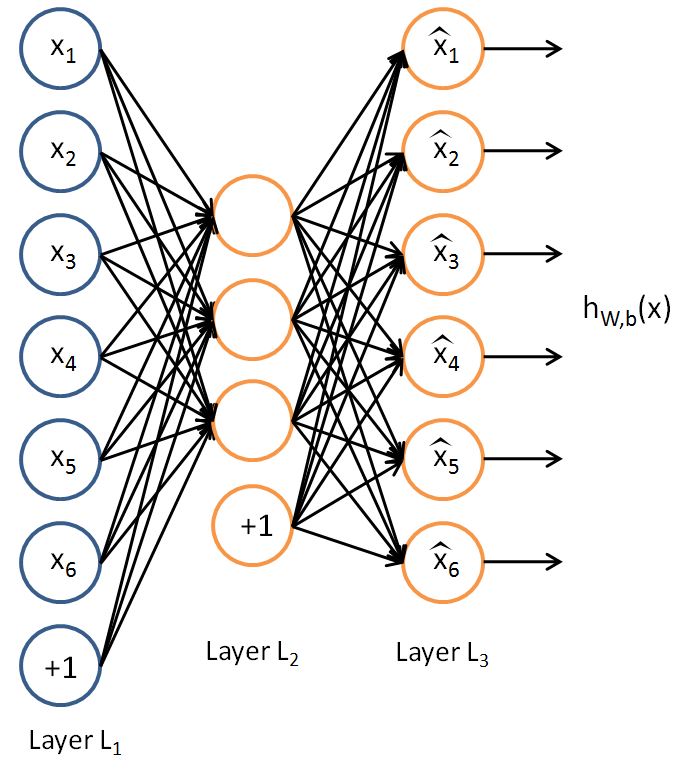
\includegraphics[width=0.5\textwidth]{figures/Autoencoder636.png}
  %\caption{}\label{fig:step1}
\end{figure}

\cnt{The autoencoder tries to learn a function $h_{W,b}(x) \approx x$. In other words, it is trying to learn an approximation to the identity function, so as to output $\hat{x}$ that is similar to $x$. The identity function seems a particularly trivial function to be trying to learn; but by placing constraints on the network, such as by limiting the number of hidden units, we can discover interesting structure about the data. As a concrete example, suppose the inputs $x$ are the pixel intensity values from a $10 \times 10$ image (100 pixels) so $n=100$, and there are $s_2=50$ hidden units in layer $L_2$. Note that we also have $y \in \Re^{100}$. Since there are only 50 hidden units, the network is forced to learn a compressed representation of the input. I.e., given only the vector of hidden unit activations $a^{(2)} \in \Re^{50}$, it must try to reconstruct the 100-pixel input $x$. If the input were completely random---say, each $x_i$ comes from an IID Gaussian independent of the other features---then this compression task would be very difficult. But if there is structure in the data, for example, if some of the input features are correlated, then this algorithm will be able to discover some of those correlations. In fact, this simple autoencoder often ends up learning a low-dimensional representation very similar to PCAs.}
    {自编码神经网络尝试学习一个 $h_{W,b}(x) \approx x$ 的函数。换句话说,它尝试逼近一个恒等函数,从而使得输出 $\hat{x}$ 接近于输入 $x$。恒等函数虽然看上去不太有学习的意义,但是当我们为自编码神经网络加入某些限制,比如限定隐藏神经元的数量,我们就可以从输入数据中发现一些有趣的结构。举例来说,假设某个自编码神经网络的输入 $x$ 是一张 $10 \times 10$ 图像(共100个像素)的像素灰度值,于是 $n=100$,其隐藏层 $L_2$ 中有 $50$ 个隐藏神经元。注意,输出也是100维的 $y \in \Re^{100}$。由于只有50个隐藏神经元,我们迫使自编码神经网络去学习输入数据的压缩表示,也就是说,它必须从50维的隐藏神经元激活度向量 $a^{(2)} \in \Re^{50}$ 中重构出100维的像素灰度值输入 $x$。如果网络的输入数据是完全随机的,比如每一个输入 $x_i$ 都是一个跟其它特征完全无关的独立同分布高斯随机变量,那么这一压缩表示将会非常难学习。但是如果输入数据中隐含着一些特定的结构,比如某些输入特征是彼此相关的,那么这一算法就可以发现输入数据中的这些相关性。事实上,这一简单的自编码神经网络通常可以学习出一个跟主元分析(PCA)结果非常相似的输入数据的低维表示。}
    {}


\cnt{Our argument above relied on the number of hidden units $s_2$ being small. But even when the number of hidden units is large (perhaps even greater than the number of input pixels), we can still discover interesting structure, by imposing other constraints on the network. In particular, if we impose a sparsity constraint on the hidden units, then the autoencoder will still discover interesting structure in the data, even if the number of hidden units is large.}
    {我们刚才的论述是基于隐藏神经元数量较小的假设。但是即使隐藏神经元的数量较大(可能比输入像素的个数还要多),我们仍然通过给自编码神经网络施加一些其他的限制条件来发现输入数据中的结构。具体来说,如果我们给隐藏神经元加入稀疏性限制,那么自编码神经网络即使在隐藏神经元数量较多的情况下仍然可以发现输入数据中一些有趣的结构。}
    {}

\cnt{Informally, we will think of a neuron as being ``active" (or as ``firing") if its output value is close to 1, or as being ``inactive" if its output value is close to 0. We would like to constrain the neurons to be inactive most of the time. This discussion assumes a sigmoid activation function. If you are using a tanh activation function, then we think of a neuron as being inactive when it outputs values close to -1.}
    {稀疏性可以被简单地解释如下。如果当神经元的输出接近于1的时候我们认为它被激活,而输出接近于0的时候认为它被抑制,那么使得神经元大部分的时间都是被抑制的限制则被称作稀疏性限制。这里我们假设的神经元的激活函数是sigmoid函数。如果你使用tanh作为激活函数的话,当神经元输出为-1的时候,我们认为神经元是被抑制的。}
    {}

\cnt{Recall that $a^{(2)}_j$ denotes the activation of hidden unit $j$ in the autoencoder. However, this notation doesn't make explicit what was the input $x$ that led to that activation. Thus, we will write $a^{(2)}_j(x)$ to denote the activation of this hidden unit when the network is given a specific input $x$. Further, let}
    {注意到 $a^{(2)}_j$ 表示隐藏神经元 $j$ 的激活度,但是这一表示方法中并未明确指出哪一个输入 $x$ 带来了这一激活度。所以我们将使用 $a^{(2)}_j(x)$ 来表示在给定输入为 $x$ 情况下,自编码神经网络隐藏神经元 $j$ 的激活度。 进一步,让}
    {}
\begin{align} \hat\rho_j = \frac{1}{m} \sum_{i=1}^m \left[ a^{(2)}_j(x^{(i)}) \right] \end{align}
\cnt{be the average activation of hidden unit $j$ (averaged over the training set). We would like to (approximately) enforce the constraint}
    {表示隐藏神经元 $j$ 的平均活跃度(在训练集上取平均)。我们可以近似的加入一条限制}
    {}
\begin{align} \hat\rho_j = \rho, \end{align}
\cnt{where $\rho$ is a sparsity parameter, typically a small value close to zero (say $\rho = 0.05$). In other words, we would like the average activation of each hidden neuron $j$ to be close to 0.05 (say). To satisfy this constraint, the hidden unit's activations must mostly be near 0.}
    {其中, $\rho$ 是稀疏性参数,通常是一个接近于0的较小的值(比如 $\rho = 0.05$)。换句话说,我们想要让隐藏神经元 $j$ 的平均活跃度接近0.05。为了满足这一条件,隐藏神经元的活跃度必须接近于0。}
    {}

\cnt{To achieve this, we will add an extra penalty term to our optimization objective that penalizes $\hat\rho_j$ deviating significantly from $\rho$. Many choices of the penalty term will give reasonable results. We will choose the following:}
    {为了实现这一限制,我们将会在我们的优化目标函数中加入一个额外的惩罚因子,而这一惩罚因子将惩罚那些 $\hat\rho_j$ 和 $\rho$ 有显著不同的情况从而使得隐藏神经元的平均活跃度保持在较小范围内。惩罚因子的具体形式有很多种合理的选择,我们将会选择以下这一种: }
    {}
\begin{align} \sum_{j=1}^{s_2} \rho \log \frac{\rho}{\hat\rho_j} + (1-\rho) \log \frac{1-\rho}{1-\hat\rho_j}. \end{align}

\cnt{Here, $s_2$ is the number of neurons in the hidden layer, and the index $j$ is summing over the hidden units in our network. If you are familiar with the concept of KL divergence, this penalty term is based on it, and can also be written}
    {这里, $s_2$ 是隐藏层中隐藏神经元的数量,而索引 $j$ 依次代表隐藏层中的每一个神经元。如果你对相对熵(KL divergence)比较熟悉,这一惩罚因子实际上是基于它的。于是惩罚因子也可以被表示为}
    {}
\begin{align} \sum_{j=1}^{s_2} {\rm KL}(\rho || \hat\rho_j), \end{align} 
\cnt{where ${\rm KL}(\rho || \hat\rho_j) = \rho \log \frac{\rho}{\hat\rho_j} + (1-\rho) \log \frac{1-\rho}{1-\hat\rho_j}$ is the Kullback-Leibler (KL) divergence between a Bernoulli random variable with mean $\rho$ and a Bernoulli random variable with mean $\hat\rho_j$. KL-divergence is a standard function for measuring how different two different distributions are. (If you've not seen KL-divergence before, don't worry about it; everything you need to know about it is contained in these notes.)}
    {其中 ${\rm KL}(\rho || \hat\rho_j) = \rho \log \frac{\rho}{\hat\rho_j} + (1-\rho) \log \frac{1-\rho}{1-\hat\rho_j}$ 是一个以 $\rho$ 为均值和一个以 $\hat\rho_j$ 为均值的两个伯努利随机变量之间的相对熵。相对熵是一种标准的用来测量两个分布之间差异的方法。(如果你没有见过相对熵,不用担心,所有你需要知道的内容都会被包含在这份笔记之中。)}
    {}

\cnt{This penalty function has the property that ${\rm KL}(\rho || \hat\rho_j) = 0$ if $\hat\rho_j = \rho$, and otherwise it increases monotonically as $\hat\rho_j$ diverges from $\rho$. For example, in the figure below, we have set $\rho = 0.2$, and plotted ${\rm KL}(\rho || \hat\rho_j)$ for a range of values of $\hat\rho_j$:}
    {这一惩罚因子有如下性质,当 $\hat\rho_j = \rho$ 时 ${\rm KL}(\rho || \hat\rho_j) = 0$,并且随着 $\hat\rho_j$ 与 $\rho$ 之间的差异增大而单调递增。举例来说,在下图中,我们设定 $\rho = 0.2$ 并且画出了相对熵值 ${\rm KL}(\rho || \hat\rho_j)$ 随着 $\hat\rho_j$ 变化的变化。}
    {}

\begin{figure}[ht] \centering
  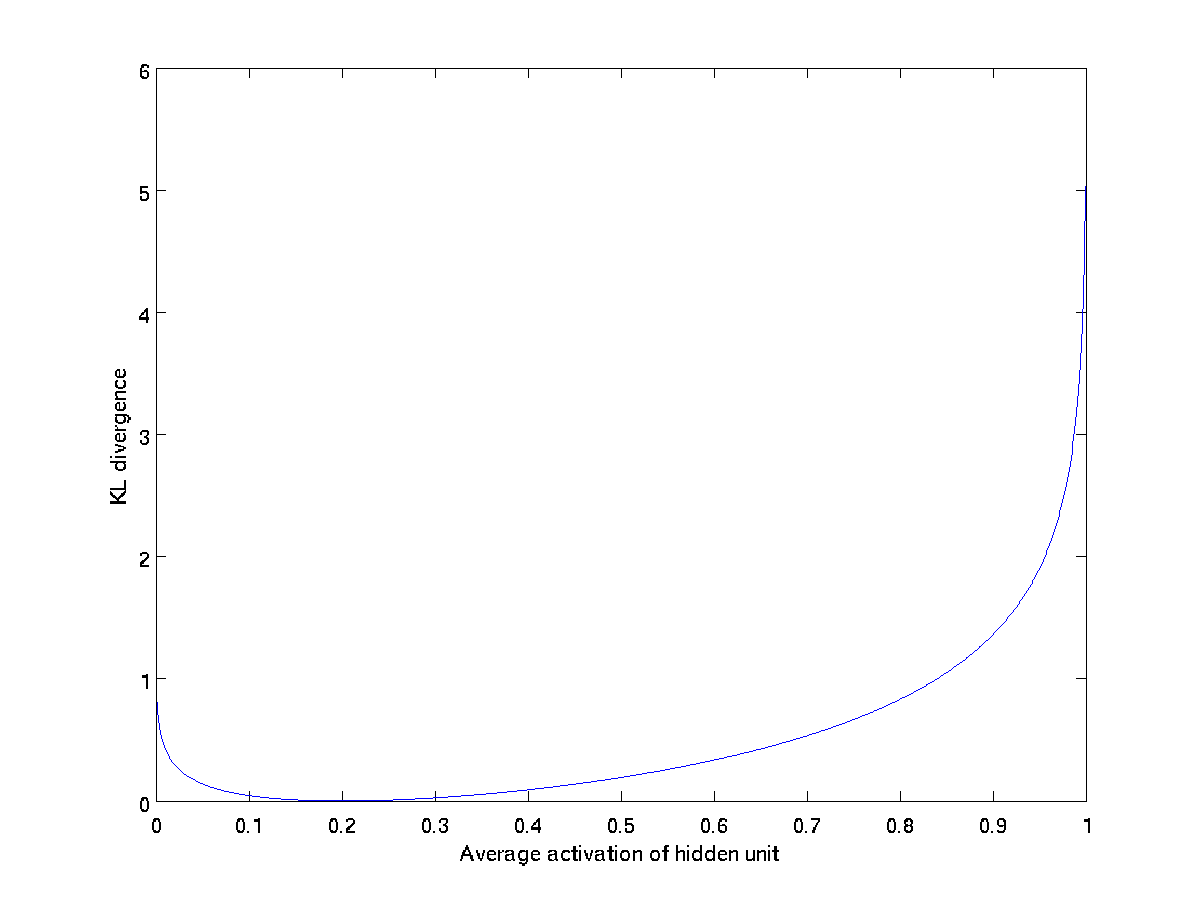
\includegraphics[width=0.8\textwidth]{figures/KLPenaltyExample.png}
  %\caption{}\label{fig:step1}
\end{figure}


\cnt{We see that the KL-divergence reaches its minimum of 0 at $\hat\rho_j = \rho$, and blows up (it actually approaches $\infty$) as $\hat\rho_j$ approaches $0$ or $1$. Thus, minimizing this penalty term has the effect of causing $\hat\rho_j$ to be close to $\rho$.}
    {我们可以看出,相对熵在 $\hat\rho_j = \rho$ 时达到它的最小值0,而当 $\hat\rho_j$ 靠近0或者1的时候,相对熵则变得非常大(其实是趋向于 $\infty$)。所以,最小化这一惩罚因子具有使得 $\hat\rho_j$ 靠近 $\rho$ 的效果。}
    {}


\cnt{Our overall cost function is now}
    {现在,我们的总体代价函数可以表示为}
    {}
\begin{align} J_{\rm sparse}(W,b) = J(W,b) + \beta \sum_{j=1}^{s_2} {\rm KL}(\rho || \hat\rho_j), \end{align}
\cnt{where $J(W,b)$ is as defined previously, and $\beta$ controls the weight of the sparsity penalty term. The term $\hat\rho_j$ (implicitly) depends on $W,b$ also, because it is the average activation of hidden unit $j$, and the activation of a hidden unit depends on the parameters $W,b$.}
    {其中 $J(W,b)$ 如之前所定义,而 $\beta$ 控制稀疏性惩罚因子的权重。 $\hat\rho_j$ 项则也(间接地)取决于 $W,b$,因为它是隐藏神经元 $j$ 的平均激活度,而隐藏层神经元的激活度取决于 $W,b$。}
    {}

\cnt{To incorporate the KL-divergence term into your derivative calculation, there is a simple-to-implement trick involving only a small change to your code. Specifically, where previously for the second layer ($l=2$), during backpropagation you would have computed}
    {为了对相对熵进行导数计算,我们可以使用一个易于实现的技巧,这只需要在你的程序中稍作改动即可。具体来说,前面在后向传播算法中计算第二层( $l=2$ )更新的时候我们已经计算了}
    {}
\begin{align} \delta^{(2)}_i = \left( \sum_{j=1}^{s_{2}} W^{(2)}_{ji} \delta^{(3)}_j \right) f'(z^{(2)}_i), \end{align} 
\cnt{now instead compute}
    {现在我们将其换成}
    {}
\begin{align} \delta^{(2)}_i = \left( \left( \sum_{j=1}^{s_{2}} W^{(2)}_{ji} \delta^{(3)}_j \right) + \beta \left( - \frac{\rho}{\hat\rho_i} + \frac{1-\rho}{1-\hat\rho_i} \right) \right) f'(z^{(2)}_i) . \end{align} 
\cnt{}{就可以了。}{}


\cnt{One subtlety is that you'll need to know $\hat\rho_i$ to compute this term. Thus, you'll need to compute a forward pass on all the training examples first to compute the average activations on the training set, before computing backpropagation on any example. If your training set is small enough to fit comfortably in computer memory (this will be the case for the programming assignment), you can compute forward passes on all your examples and keep the resulting activations in memory and compute the $\hat\rho_is$. Then you can use your precomputed activations to perform backpropagation on all your examples. If your data is too large to fit in memory, you may have to scan through your examples computing a forward pass on each to accumulate (sum up) the activations and compute $\hat\rho_i$ (discarding the result of each forward pass after you have taken its activations $a^{(2)}_i$ into account for computing $\hat\rho_i$). Then after having computed $\hat\rho_i$, you'd have to redo the forward pass for each example so that you can do backpropagation on that example. In this latter case, you would end up computing a forward pass twice on each example in your training set, making it computationally less efficient.}
    {有一个需要注意的地方就是我们需要知道 $\hat\rho_i$ 来计算这一项更新。所以在计算任何神经元的后向传播之前,你需要对所有的训练样本计算一遍前向传播,从而获取平均激活度。如果你的训练样本可以小到被整个存到内存之中(对于编程作业来说,通常如此),你可以方便地在你所有的样本上计算前向传播并将得到的激活度存入内存并且计算平均激活度 。然后你就可以使用事先计算好的激活度来对所有的训练样本进行后向传播的计算。如果你的数据量太大,无法全部存入内存,你就可以扫过你的训练样本并计算一次前向传播,然后将获得的结果累积起来并计算平均激活度 $\hat\rho_i$ (当某一个前向传播的结果中的激活度 $a^{(2)}_i$ 被用于计算平均激活度 $\hat\rho_i$ 之后就可以将此结果删除)。然后当你完成平均激活度 $\hat\rho_i$ 的计算之后,你需要重新对每一个训练样本做一次前向传播从而可以对其进行后向传播的计算。对于后一种情况,你对每一个训练样本需要计算两次前向传播,所以在计算上的效率会稍低一些。}
    {}

\cnt{The full derivation showing that the algorithm above results in gradient descent is beyond the scope of these notes. But if you implement the autoencoder using backpropagation modified this way, you will be performing gradient descent exactly on the objective $J_{\rm sparse}(W,b)$. Using the derivative checking method, you will be able to verify this for yourself as well.}
    {证明上面算法能达到梯度下降效果的完整推导过程不再本教程的范围之内。不过如果你想要使用经过以上修改的后向传播来实现自编码神经网络,那么你就会对目标函数 $J_{\rm sparse}(W,b)$ 做梯度下降。使用梯度验证方法,你可以自己来验证梯度下降算法是否正确。}
    {}

\subsection{\cnt{Visualizing a Trained Autoencoder}{可视化自编码器训练结果}{}}

\cnt{Having trained a (sparse) autoencoder, we would now like to visualize the function learned by the algorithm, to try to understand what it has learned. Consider the case of training an autoencoder on $10 \times 10$ images, so that $n = 100$. Each hidden unit $i$ computes a function of the input:}
    {训练完(稀疏)自编码器,我们还想把这自编码器学到的函数可视化出来,好弄明白它到底学到了什么。我们以在$10 \times 10$图像(即n=100)上训练自编码器为例。在该自编码器中,每个隐藏单元i对如下关于输入的函数进行计算:}
    {}
\begin{align} a^{(2)}_i = f\left(\sum_{j=1}^{100} W^{(1)}_{ij} x_j + b^{(1)}_i \right). \end{align} 

\cnt{We will visualize the function computed by hidden unit $i$ --- which depends on the parameters $W^{(1)}_{ij}$ (ignoring the bias term for now)---using a 2D image. In particular, we think of $a^{(2)}_i$ as some non-linear feature of the input $x$. We ask: What input image $x$ would cause $a^{(2)}_i$ to be maximally activated? (Less formally, what is the feature that hidden unit $i$ is looking for?) For this question to have a non-trivial answer, we must impose some constraints on $x$. If we suppose that the input is norm constrained by $||x||^2 = \sum_{i=1}^{100} x_i^2 \leq 1$, then one can show (try doing this yourself) that the input which maximally activates hidden unit $i$ is given by setting pixel $x_j$ (for all 100 pixels, $j=1,\ldots, 100$) to}
    {我们将要可视化的函数,就是上面这个以2D图像为输入、并由隐藏单元i计算出来的函数。它是依赖于参数 $W^{(1)}_{ij}$ 的(暂时忽略偏置项 $b_i$)。需要注意的是,$a^{(2)}_i$ 可看作输入 $x$ 的非线性特征。不过还有个问题:什么样的输入图像 $x$ 可让 $a^{(2)}_i$ 得到最大程度的激励?(通俗一点说,隐藏单元 $i$ 要找个什么样的特征?)。这里我们必须给 $x$ 加约束,否则会得到平凡解。若假设输入有范数约束 $||x||^2 = \sum_{i=1}^{100} x_i^2 \leq 1$,则可证(请读者自行推导)令隐藏单元 $i$ 得到最大激励的输入应由下面公式计算的像素 $x_j$ 给出(共需计算100个像素,$j=1,\ldots, 100$):}
    {}
\begin{align} x_j = \frac{W^{(1)}_{ij}}{\sqrt{\sum_{j=1}^{100} (W^{(1)}_{ij})^2}}. \end{align} 

\cnt{By displaying the image formed by these pixel intensity values, we can begin to understand what feature hidden unit $i$ is looking for.}
    {当我们用上式算出各像素的值、把它们组成一幅图像、并将图像呈现在我们面前之时,隐藏单元 $i$ 所追寻特征的真正含义也渐渐明朗起来。}
    {}

\cnt{If we have an autoencoder with 100 hidden units (say), then we our visualization will have 100 such images---one per hidden unit. By examining these 100 images, we can try to understand what the ensemble of hidden units is learning.}
    {假如我们训练的自编码器有100个隐藏单元,可视化结果就会包含100幅这样的图像——每个隐藏单元都对应一幅图像。审视这100幅图像,我们可以试着体会这些隐藏单元学出来的整体效果是什么样的。}
    {}


\cnt{When we do this for a sparse autoencoder (trained with 100 hidden units on 10x10 pixel inputs)}
    {当我们对稀疏自编码器进行上述可视化处理之后(100个隐藏单元,在10X10像素的输入上训练),}
    {}
\footnote{
\cnt{The learned features were obtained by training on \emph{whitened} natural images. Whitening is a preprocessing step which removes redundancy in the input, by causing adjacent pixels to become less correlated.}
    {}
    {}
}
\cnt{we get the following result:}
    {结果如下所示:}
    {}

\begin{figure}[ht] \centering
  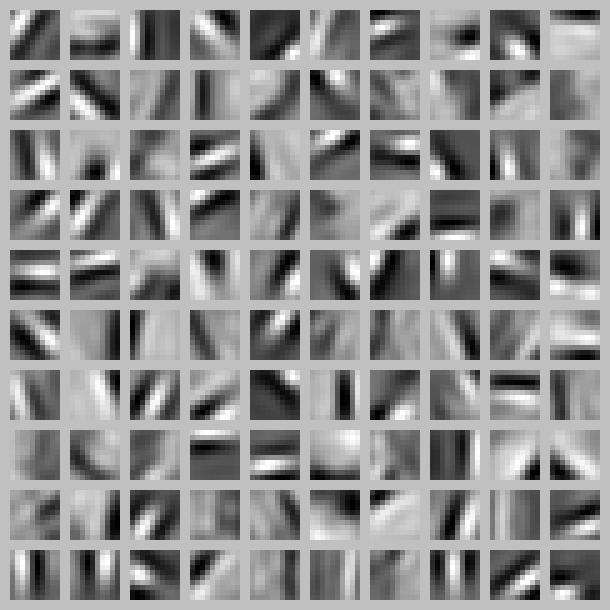
\includegraphics[width=0.5\textwidth]{figures/ExampleSparseAutoencoderWeights.png}
  %\caption{}\label{fig:step1}
\end{figure}

\cnt{Each square in the figure above shows the (norm bounded) input image $x$ that maximally actives one of 100 hidden units. We see that the different hidden units have learned to detect edges at different positions and orientations in the image.}
    {上图的每个小方块都给出了一个(带有有界范数 的)输入图像 $x$,它可使这100个隐藏单元中的某一个获得最大激励。我们可以看到,不同的隐藏单元学会了在图像的不同位置和方向进行边缘检测。}
    {}


\cnt{These features are, not surprisingly, useful for such tasks as object recognition and other vision tasks. When applied to other input domains (such as audio), this algorithm also learns useful representations/features for those domains too.}
    {显而易见,这些特征对物体识别等计算机视觉任务是十分有用的。若将其用于其他输入域(如音频),该算法也可学到对这些输入域有用的表示或特征。}
    {}

\subsection{\cnt{Sparse Autoencoder Notation Summary}{稀疏自编码器符号一览表}{}}

\cnt{Here is a summary of the symbols used in our derivation of the sparse autoencoder:}
    {下面是我们在推导sparse autoencoder时使用的符号一览表:}
    {}

\begin{longtable}[h]{>{\centering\arraybackslash}m{0.1\textwidth}m{0.7\textwidth}}
\caption{\cnt{Sparse Autoencoder Notation Summary}{稀疏自编码器符号一览表}{}} \label{tab:sparseautoencodersummary}\\
\toprule
\textbf{\cnt{Symbol}{符号}{}}&\textbf{\cnt{Meaning}{含义}{}} \\
\midrule
\endfirsthead  % endfirsthead 以上內容只出現在第一頁
\midrule
\textbf{\cnt{Symbol}{符号}{}}&\textbf{\cnt{Meaning}{含义}{}} \\
\midrule
\endhead % endfirsthead 及 endhead 間的內容會排版至每頁上方
%\midrule
\multicolumn{2}{r}{\cnt{To be continued}{续下页}{} \dots} \\
\midrule

\endfoot % endfoot 以上的內會出現在每頁底部
\endlastfoot

$x$	& \cnt{Input features for a training example, $x \in \Re^{n}$.}{训练样本的输入特征,$x \in \Re^{n}$.}{} \\
  \midrule

$y$	& \cnt{Output/target values. Here, $y$ can be vector valued. In the case of an autoencoder, $y=x$.}{输出值/目标值. 这里 $y$ 可以是向量. 在autoencoder中,$y=x$.}{} \\
  \midrule

$(x^{(i)}, y^{(i)})$	& \cnt{The $i$-th training example}{第 $i$ 个训练样本}{} \\
  \midrule

$h_{W,b}(x)$	& \cnt{Output of our hypothesis on input $x$, using parameters $W,b$. This should be a vector of the same dimension as the target value $y$.}{输入为 $x$ 时的假设输出,其中包含参数 $W,b$. 该输出应当与目标值 $y$ 具有相同的维数.}{} \\
  \midrule

$W^{(l)}_{ij}$	& \cnt{The parameter associated with the connection between unit $j$ in layer $l$, and unit $i$ in layer $l+1$.}{连接第 $l$ 层 $j$ 单元和第 $l+1$ 层 $i$ 单元的参数.}{} \\
  \midrule

$b^{(l)}_{i}$	& \cnt{The bias term associated with unit $i$ in layer $l+1$. Can also be thought of as the parameter associated with the connection between the bias unit in layer $l$ and unit $i$ in layer $l+1$.}{第 $l+1$ 层 $i$ 单元的偏置项. 也可以看作是连接第 $l$ 层偏置单元和第 $l+1$ 层 $i$ 单元的参数.}{} \\
  \midrule

$\theta$	& \cnt{Our parameter vector. It is useful to think of this as the result of taking the parameters $W,b$ and ``unrolling them into a long column vector.}{参数向量. 可以认为该向量是通过将参数 $W,b$ 组合展开为一个长的列向量而得到.}{} \\
  \midrule

$a^{(l)}_i$	& \cnt{Activation (output) of unit $i$ in layer $l$ of the network. In addition, since layer $L_1$ is the input layer, we also have $a^{(1)}_i = x_i$.}{网络中第 $l$ 层 $i$ 单元的激活(输出)值. 另外,由于 $L_1$ 层是输入层,所以 $a^{(1)}_i = x_i$.}{} \\
  \midrule

$f(\cdot)$	& \cnt{The activation function. Throughout these notes, we used $f(z) = \tanh(z)$.}{激活函数. 本文中我们使用 $f(z) = \tanh(z)$.}{} \\
  \midrule

$z^{(l)}_i$	& \cnt{Total weighted sum of inputs to unit $i$ in layer $l$. Thus, $a^{(l)}_i = f(z^{(l)}_i)$.}{第 $l$ 层 $i$ 单元所有输入的加权和. 因此有 $a^{(l)}_i = f(z^{(l)}_i)$.}{} \\
  \midrule

$\alpha$	& \cnt{Learning rate parameter}{学习率}{} \\
  \midrule

$s_l$	& \cnt{Number of units in layer $l$ (not counting the bias unit).}{第 $l$ 层的单元数目(不包含偏置单元).}{} \\
  \midrule

$n_l$	& \cnt{Number layers in the network. Layer $L_1$ is usually the input layer, and layer $L_{n_l}$ the output layer.}{网络中的层数. 通常 $L_1$ 层是输入层,$L_{n_l}$ 层是输出层.}{} \\
  \midrule

$\lambda$	& \cnt{Weight decay parameter.}{权重衰减系数.}{} \\
  \midrule

$\hat{x}$	& \cnt{For an autoencoder, its output; i.e., its reconstruction of the input $x$. Same meaning as $h_{W,b}(x)$.}{对于一个autoencoder,该符号表示其输出值;亦即输入值 $x$ 的重构值. 与 $h_{W,b}(x)$ 含义相同.}{} \\
  \midrule

$\rho$	& \cnt{Sparsity parameter, which specifies our desired level of sparsity}{稀疏值,可以用它指定我们所需的稀疏程度}{} \\
  \midrule

$\hat\rho_i$	& \cnt{The average activation of hidden unit $i$ (in the sparse autoencoder).}{(sparse autoencoder中)隐藏单元 $i$ 的平均激活值.}{} \\
  \midrule

$\beta$	& \cnt{Weight of the sparsity penalty term (in the sparse autoencoder objective).}{(sparse autoencoder目标函数中)稀疏值惩罚项的权重.}{} \\

\bottomrule
\end{longtable}

\subsection{\cnt{Exercise: Sparse Autoencoder}{练习:稀疏自编码器}{}} \label{chp:execsparseautoenc}


\cnt{You may want to download the related document from \url{http://nlp.stanford.edu/~socherr/sparseAutoencoder_2011new.pdf} and \url{http://www.stanford.edu/class/cs294a/cs294a_2011-assignment.pdf}.}
    {可以从 \url{http://nlp.stanford.edu/~socherr/sparseAutoencoder_2011new.pdf} 和 \url{http://www.stanford.edu/class/cs294a/cs294a_2011-assignment.pdf} 下载文档。}
    {}

\textbf{\cnt{Sparse autoencoder implementation}{稀疏自编码器的实现}{}}

\cnt{In this problem set, you will implement the sparse autoencoder algorithm, and show how it discovers that edges are a good representation for natural images. (Images provided by Bruno Olshausen.) The sparse autoencoder algorithm is described in the lecture notes found on the course website. }
    {}
    {}


\cnt{In the file
%\href{http://ufldl.stanford.edu/wiki/resources/sparseae_exercise.zip}{sparseae_exercise.zip}
\url{http://ufldl.stanford.edu/wiki/resources/sparseae_exercise.zip}
, we have provided some starter code in Matlab. You should write your code at the places indicated in the files (\texttt{``YOUR CODE HERE"}). You have to complete the following files: \texttt{sampleIMAGES.m, sparseAutoencoderCost.m, computeNumericalGradient.m}. The starter code in \texttt{train.m} shows how these functions are used.}
    {}
    {}


\cnt{Specifically, in this exercise you will implement a sparse autoencoder, trained with $8 \times 8$ image patches using the L-BFGS optimization algorithm.}
    {}
    {}


\cnt{\emph{A note on the software}: The provided .zip file includes a subdirectory \texttt{minFunc} with 3rd party software implementing L-BFGS, that is licensed under a Creative Commons, Attribute, Non-Commercial license. If you need to use this software for commercial purposes, you can download and use a different function (fminlbfgs) that can serve the same purpose, but runs $~ 3 \times $ slower for this exercise (and thus is less recommended). You can read more about this in the
%\href{http://deeplearning.stanford.edu/wiki/index.php/Fminlbfgs_Details}{Fminlbfgs_Details}
\url{http://deeplearning.stanford.edu/wiki/index.php/Fminlbfgs_Details}
page.}
    {}
    {}


\subsubsection{\cnt{Step 1: Generate training set}{第一步:生成训练集}{}}

\cnt{The first step is to generate a training set. To get a single training example $x$, randomly pick one of the 10 images, then randomly sample an $8 \times 8$ image patch from the selected image, and convert the image patch (either in row-major order or column-major order; it doesn't matter) into a 64-dimensional vector to get a training example $x \in \Re^{64}$.}
    {}
    {}

\cnt{Complete the code in \texttt{sampleIMAGES.m}. Your code should sample 10000 image patches and concatenate them into a $64 \times 10000$ matrix. }
    {}
    {}

\cnt{To make sure your implementation is working, run the code in ``Step 1" of train.m. This should result in a plot of a random sample of 200 patches from the dataset.}
    {}
    {}

\cnt{\emph{Implementational tip}: When we run our implemented \texttt{sampleImages()}, it takes under 5 seconds. If your implementation takes over 30 seconds, it may be because you are accidentally making a copy of an entire $512 \times 512$ image each time you're picking a random image. By copying a $512 \times 512$ image 10000 times, this can make your implementation much less efficient. While this doesn't slow down your code significantly for this exercise (because we have only 10000 examples), when we scale to much larger problems later this quarter with $10^6$ or more examples, this will significantly slow down your code. Please implement \texttt{sampleIMAGES} so that you aren't making a copy of an entire $512 \times 512$ image each time you need to cut out an $8 \times 8$ image patch. }
    {}
    {}

\subsubsection{\cnt{Step 2: Sparse autoencoder objective}{第二步:稀疏自编码器}{}}

\cnt{Implement code to compute the sparse autoencoder cost function $J_{sparse}(W,b)$ (Section 3 of the lecture notes) and the corresponding derivatives of $J_{sparse}$ with respect to the different parameters. Use the sigmoid function for the activation function, $f(z) = \frac{1}{{1+e^{-z}}}$. In particular, complete the code in \texttt{sparseAutoencoderCost.m}. }
    {}
    {}

\cnt{The sparse autoencoder is parameterized by matrices $W^{(1)} \in \Re^{s_1\times s_2}, W^{(2)} \in \Re^{s_2\times s_3}$ vectors $b^{(1)} \in \Re^{s_2}, b^{(2)} \in \Re^{s_3}$. However, for subsequent notational convenience, we will ``unroll" all of these parameters into a very long parameter vector $\theta$ with $s_1s_2 + s_2s_3 + s_2 + s_3$ elements. The code for converting between the $(W^{(1)},W^{(2)},b^{(1)},b^{(2)})$ and the $\theta$ parameterization is already provided in the starter code.}
    {}
    {}



\cnt{\emph{Implementational tip}: The objective $J_{sparse}(W,b)$ contains 3 terms, corresponding to the squared error term, the weight decay term, and the sparsity penalty. You're welcome to implement this however you want, but for ease of debugging, you might implement the cost function and derivative computation (backpropagation) only for the squared error term first (this corresponds to setting $\lambda = \beta = 0$), and implement the gradient checking method in the next section to first verify that this code is correct. Then only after you have verified that the objective and derivative calculations corresponding to the squared error term are working, add in code to compute the weight decay and sparsity penalty terms and their corresponding derivatives. }
    {}
    {}


\subsubsection{\cnt{Step 3: Gradient checking}{第三步:梯度检测}{}}

\cnt{Following Section 2.3 of the lecture notes, implement code for gradient checking. Specifically, complete the code in \texttt{computeNumericalGradient.m}. Please use ${\rm EPSILON} = 10^{-4}$ as described in the lecture notes.}
    {}
    {}

\cnt{We've also provided code in checkNumericalGradient.m for you to test your code. This code defines a simple quadratic function $h: \Re^2 \mapsto \Re$ given by $h(x) = x_1^2 + 3x_1 x_2$, and evaluates it at the point $x = (4,10)^T$. It allows you to verify that your numerically evaluated gradient is very close to the true (analytically computed) gradient.}
    {}
    {}

\cnt{After using checkNumericalGradient.m to make sure your implementation is correct, next use computeNumericalGradient.m to make sure that your sparseAutoencoderCost.m is computing derivatives correctly. For details, see Steps 3 in train.m. We strongly encourage you not to proceed to the next step until you've verified that your derivative computations are correct. }
    {}
    {}

\cnt{\emph{Implementational tip}: If you are debugging your code, performing gradient checking on smaller models and smaller training sets (e.g., using only 10 training examples and 1-2 hidden units) may speed things up. }
    {}
    {}

\subsubsection{\cnt{Step 4: Train the sparse autoencoder}{第四步:训练稀疏自编码器}{}}

\cnt{Now that you have code that computes Jsparse and its derivatives, we're ready to minimize Jsparse with respect to its parameters, and thereby train our sparse autoencoder. }
    {}
    {}

\cnt{We will use the L-BFGS algorithm. This is provided to you in a function called minFunc (code provided by Mark Schmidt) included in the starter code. (For the purpose of this assignment, you only need to call minFunc with the default parameters. You do not need to know how L-BFGS works.) We have already provided code in train.m (Step 4) to call minFunc. The minFunc code assumes that the parameters to be optimized are a long parameter vector; so we will use the ``$\theta$" parameterization rather than the ``$(W^{(1)},W^{(2)},b^{(1)},b^{(2)})$" parameterization when passing our parameters to it. }
    {}
    {}

\cnt{Train a sparse autoencoder with 64 input units, 25 hidden units, and 64 output units. In our starter code, we have provided a function for initializing the parameters. We initialize the biases $b^{(l)}_i$ to zero, and the weights $W^{(l)}_{ij}$ to random numbers drawn uniformly from the interval $\left[-\sqrt{\dfrac{6}{n_{\rm in}+n_{\rm out}+1}},\sqrt{\dfrac{6}{n_{\rm in}+n_{\rm out}+1}}\,\right]$, where $n_{in}$ is the fan-in (the number of inputs feeding into a node) and $n_{out}$ is the fan-in (the number of units that a node feeds into). }
    {}
    {}

\cnt{The values we provided for the various parameters ($\lambda ,\beta ,\rho$, etc.) should work, but feel free to play with different settings of the parameters as well.}
    {}
    {}

\cnt{\emph{Implementational tip}: Once you have your backpropagation implementation correctly computing the derivatives (as verified using gradient checking in Step 3), when you are now using it with L-BFGS to optimize $J_{sparse}(W,b)$, make sure you're not doing gradient-checking on every step. Backpropagation can be used to compute the derivatives of Jsparse(W,b) fairly efficiently, and if you were additionally computing the gradient numerically on every step, this would slow down your program significantly.}
    {}
    {}

\subsubsection{\cnt{Step 5: Visualization}{第五步:可视化}{}}

\cnt{After training the autoencoder, use \texttt{display\_network.m} to visualize the learned weights. (See \texttt{train.m}, Step 5.) Run ``\texttt{print -djpeg weights.jpg}" to save the visualization to a file ``\texttt{weights.jpg}" (which you will submit together with your code).}
    {}
    {}

\textbf{
\cnt{Results}
    {结果}
    {}
}


\cnt{To successfully complete this assignment, you should demonstrate your sparse autoencoder algorithm learning a set of edge detectors. For example, this was the visualization we obtained:}
    {}
    {}

\begin{figure}[ht] \centering
  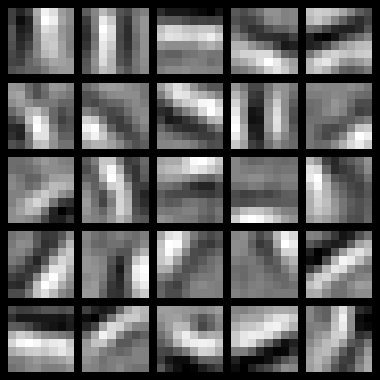
\includegraphics[width=0.5\textwidth]{figures/Gabor.jpg}
  %\caption{}\label{fig:step1}
\end{figure}

\cnt{Our implementation took around 5 minutes to run on a fast computer. In case you end up needing to try out multiple implementations or different parameter values, be sure to budget enough time for debugging and to run the experiments you'll need.}
    {}
    {}

\cnt{Also, by way of comparison, here are some visualizations from implementations that we do not consider successful (either a buggy implementation, or where the parameters were poorly tuned):}
    {}
    {}

\begin{figure}[ht] \centering
  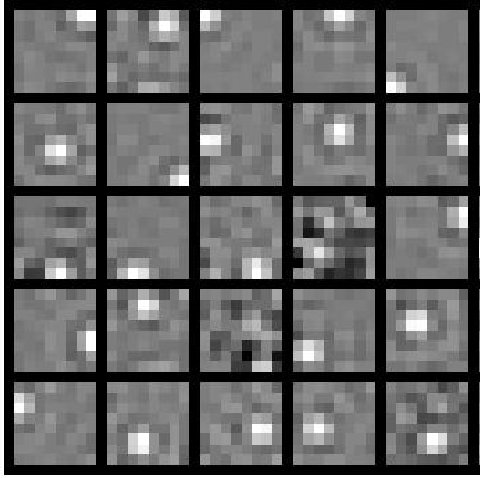
\includegraphics[width=0.3\textwidth]{figures/Badfilter1.jpg}
  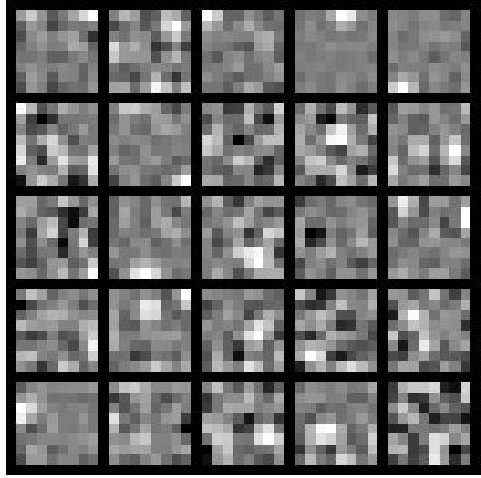
\includegraphics[width=0.3\textwidth]{figures/Badfilter2.jpg}
  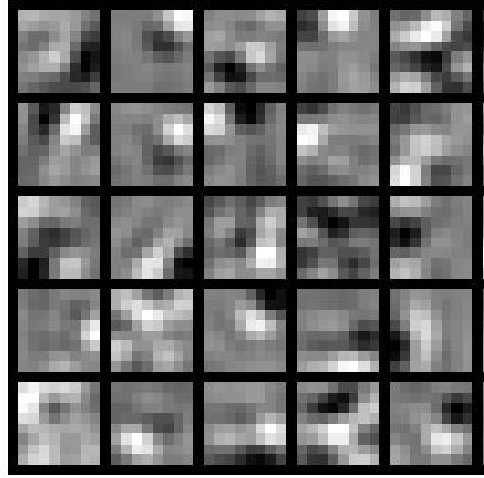
\includegraphics[width=0.3\textwidth]{figures/Badfilter3.jpg}
  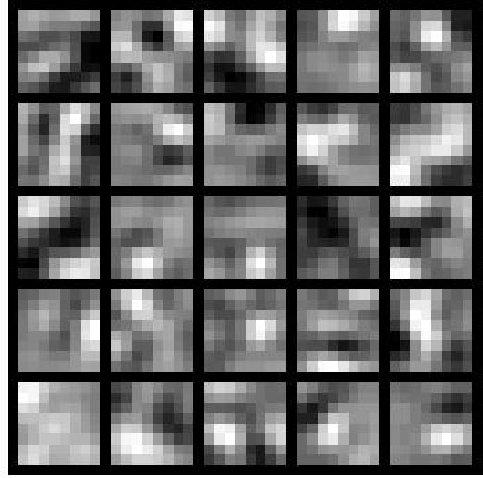
\includegraphics[width=0.3\textwidth]{figures/Badfilter4.jpg}
  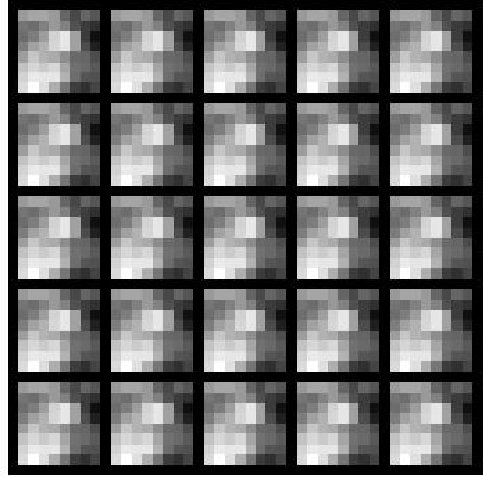
\includegraphics[width=0.3\textwidth]{figures/Badfilter5.jpg}
  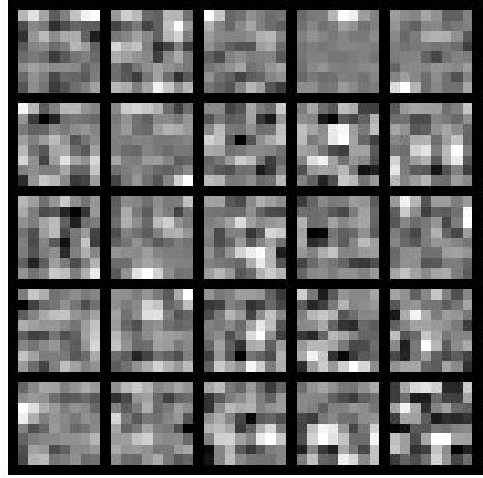
\includegraphics[width=0.3\textwidth]{figures/Badfilter6.jpg}
  %\caption{}\label{fig:step1}
\end{figure}
